\documentclass[12pt]{article}
\usepackage[utf8]{inputenc}
\usepackage[english]{babel}
\usepackage[normalem]{ulem}
\usepackage{amsmath, amsthm, amssymb, amsfonts}
\usepackage{mathtools}
\usepackage{commath}
\usepackage{bm}
\usepackage{enumerate}
\usepackage[margin = 0.75in]{geometry}
\usepackage{graphicx}

% tikz picture style
\usepackage{tikz}
\usetikzlibrary{arrows}
\usetikzlibrary{decorations.markings}
\usetikzlibrary{shapes,positioning,intersections,quotes}



\usepackage{hyperref}
\usepackage{cleveref}

\hypersetup{
	colorlinks=true,
	linkcolor=blue,
	filecolor=magenta,      
	urlcolor=cyan,
}
\usepackage{tcolorbox}
\setlength{\parskip}{0.5\baselineskip}%
\setlength{\parindent}{1cm}%


% define new command
\newcommand{\E}{\mathbb{E}}
\newcommand{\R}{\mathbb{R}}
\newcommand{\Rinf}{\mathbb{R}_{\infty}}
\newcommand{\C}{\mathbb{C}}
\newcommand{\N}{\mathbb{N}}
\newcommand{\Q}{\mathbb{Q}}
\newcommand{\Z}{\mathbb{Z}}
\newcommand{\Cinf}{\overline{\C}}
\newcommand{\zcal}{\mathcal{Z}}

\let\oldsection\section
\renewcommand\section{\clearpage\oldsection}


\theoremstyle{definition}
\newtheorem{thm}{Theorem}
\newtheorem{lem}{Lemma}
\newtheorem{cor}{Corollary}
\newtheorem{defn}{Definition}
\newtheorem{ex}{Exercise}
\newtheorem{res}{Result}
\newtheorem{prop}{Proposition}



% define theorems and lemmas
\newenvironment{definition}{
\begin{tcolorbox}[colback=green!5!white,colframe=green!75!black, parbox = false]\begin{defn} }{\end{defn}\end{tcolorbox} }

\newenvironment{theorem}{
\begin{tcolorbox}[colback=green!5!white,colframe=green!75!black, parbox = false]\begin{thm} }{\end{thm}\end{tcolorbox} }

\newenvironment{lemma}{
\begin{tcolorbox}[colback=green!5!white,colframe=green!75!black, parbox = false]\begin{lem} }{\end{lem}\end{tcolorbox} }

\newenvironment{result}{
\begin{tcolorbox}[colback=green!5!white,colframe=green!75!black, parbox = false]\begin{res} }{\end{res}\end{tcolorbox} }

\newenvironment{proposition}{
\begin{tcolorbox}[colback=green!5!white,colframe=green!75!black, parbox = false]\begin{prop} }{\end{prop}\end{tcolorbox} }

    
\newenvironment{note}{
\begin{tcolorbox}[colback=blue!5!white,colframe=blue!75!black,title=Note, parbox = false] }{\end{tcolorbox} }

\newenvironment{remark}{
\begin{tcolorbox}[colback=blue!5!white,colframe=blue!75!black,title=Remark, parbox = false] }{\end{tcolorbox} }

\newenvironment{corollary}{
\begin{tcolorbox}[colback=blue!5!white,colframe=blue!75!black, parbox = false]\begin{cor} }{\end{cor}\end{tcolorbox} }
    
\newenvironment{example}{
\begin{tcolorbox}[colback=blue!5!white,colframe=blue!75!black, title = Example, parbox = false] }{\end{tcolorbox} }
    
\newenvironment{exercise}{
\begin{tcolorbox}[colback=red!5!white,colframe=red!75!black, parbox = false]\begin{ex} }{\end{ex}\end{tcolorbox} }


\title{\LARGE \textbf{\textcolor{magenta}{Complex Analysis}}}
\author{M.Stat. $2019-2021$ Batch}
\date{\today}

\begin{document}

\maketitle
	
\begin{abstract}
    This contains some notes on Complex Analysis, taught by Dr. Paramita Das for Master of Statistics (M.Stat.) 1st Year batch 2019-20 session. During post midsem of spring $2020$ session, the classes were suspended due to a global pandemic situation created by the breakout of Coronavirus (COVID-19). This notes are intended to cover those lost classes.
\end{abstract}
\pagebreak

\tableofcontents
\pagebreak



\section{Limit and Differentiability of Complex Functions}

Throughout this section, we shall consider a complex valued function from the domain of complex numbers (or the extended complex plane), i.e. consider $$f: \C \rightarrow \C$$

\subsection{Limit of a Complex Function}

\begin{definition}
    A function $f : \C \rightarrow \C$ is said to have limit $l$, where $l \in \C$, as $z \rightarrow z_0$, if the following holds;
    $$\forall \epsilon > 0;\quad \exists \delta > 0; \text{ such that } 0 < \vert z - z_0 \vert < \delta \Rightarrow \vert f(z) - l \vert < \delta$$
    where $\vert z \vert$ denotes the absolute value of the complex number $z$.
    
    Here we denote, $$\lim_{z \rightarrow z_0} f(z) = l$$
\end{definition}

Note that, since the limit $z \rightarrow z_0$ is given through the notion $\vert z - z_0 \vert$ is infinitestimally small, the complex number $z$ can go to the complex number $z_0$ through any direction in the complex plane, in contrast to limit of real values where we have only left and right hand limits. 

In case of real values, there are two distinguishable infinites, $\infty$ or $-\infty$, and we can define limits of $x \rightarrow \infty$ or $x \rightarrow (-\infty)$. However, for complex numbers, there is only one such infinity, and it is denoted by the notion $\vert z \vert > M$, for any large positive real number $M$.

\begin{result}
    Consider the following useful results.
    \begin{enumerate}
        \item $\lim_{z \rightarrow z_0} f(z) = l \iff \lim_{z \rightarrow z_0} \bar{f(z)} = \bar{l}$, where $\bar{z}$ denotes the complex conjugate of $z$.
        \item $\lim_{z \rightarrow z_0} f(z) = l \Rightarrow \lim_{z \rightarrow z_0} \Re (f(z)) = \Re(l)$, where $\Re(z)$ denotes the real part of $z$.
        \item $\lim_{z \rightarrow z_0} f(z) = l \Rightarrow \lim_{z \rightarrow z_0} \Im(f(z)) = \Im(l)$, where $\Im(z)$ denotes the imaginary part of $z$.
    \end{enumerate}
\end{result}

\begin{definition}
    A function $f: \C \rightarrow \C$ is said to be continuous at $z_0$, if $\lim_{z \rightarrow z_0} f(z) = f(z_0)$.\par 
    If $f$ is continuous at all points of $\C$, then we say $f$ is continuous on $\C$.
\end{definition}


\subsection{Introduction to Analytic functions}

\begin{definition}
Suppose, $\Omega\subset\C$ and $f:\Omega \to \C$, $a\in \R$. $f$ is analytic at $a$ if,

\begin{equation*}
    \lim_{h\to 0}\dfrac{f(a+h)-f(a)}{h}
\end{equation*}

exists and the value of this limit is denoted by $f'(a)$.\par

If $f$ is analytic at each point of $\Omega$ then we say that $f$ is analytic on $\Omega$.\par In other words, an analytic function is a complex function of a complex variable which possesses a derivative.
\end{definition}

\begin{theorem}
    Similar to the result of real valued functions, a complex valued function $f$ is analytic at $z_0$ implies $f$ is continuous at $z_0$.
\end{theorem}

\begin{proof}
    Note that, 
    $$f(z_0+h) - f(z_0) = \left(\dfrac{f(z_0+h) - f(z_0)}{h}\right) \times h$$
    Now, taking limit as $h \rightarrow 0$, to both sides (in the notion of complex numbers), we get;
    $$\lim_{h \rightarrow 0} f(z_0+h) - f(z_0) = f'(z_0) \times \lim_{h\rightarrow 0}h = 0$$
    Rewriting $(z_0 + h)$ as any arbitrary $z$ such that $z\rightarrow z_0$, we obtain the result.
\end{proof}

Now we shall state and prove the most useful theorem in Complex Analysis.

\begin{theorem}
    Let $f:\C \rightarrow \C$ be a complex valued function. Identify $f(z) = u(z) + i v(z)$, where both $u(\cdot)$ and $v(\cdot)$ are functions from $\C$ to $\R$. 
    
    Define $\dfrac{\partial u}{\partial x}$ and $\dfrac{\partial u}{\partial y}$ to be the partial derivative of $u$ for change in real part and imaginary part of the argument respectively.
    
    Then, if $f$ is analytic at $z_0$, then we have the following:
    
    \begin{align}
        \dfrac{\partial u}{\partial x}(z_0) & =\dfrac{\partial v}{\partial y}(z_0)\\
        \dfrac{\partial u}{\partial y}(z_0) &=-\dfrac{\partial v}{\partial x}(z_0)
    \end{align}
    
    We may drop the point $z_0$, in case when there is no ambiguity. These two equations are called \textbf{Cauchy Riemann Equations}.
\end{theorem}

\begin{proof}
    To prove this, we consider $h = h_1 + ih_2$, where $h_1, h_2 \in \R$, and consider two limits in the differentiation, one from the real line, and another from the purely imaginary line.
    
    Note that,
    \begin{align*}
        f'(z_0) & = \lim_{h_1 \rightarrow 0} \dfrac{f(z_0 + h_1) - f(z_0)}{h_1}\\
        & \lim_{h_1 \rightarrow 0} \dfrac{u(z_0 + h_1) + iv(z_0 + h_1) - u(z_0) - iv(z_0)}{h_1}\\
        & = \lim_{h_1 \rightarrow 0} \dfrac{u(z_0 + h_1) - u(z_0)}{h_1} + i\lim_{h_1 \rightarrow 0} \dfrac{v(z_0 + h_1) - v(z_0)}{h_1}\\
        & = \dfrac{\partial u}{\partial x} + i \dfrac{\partial v}{\partial x}
    \end{align*}
    
    Similarly,
    \begin{align*}
        f'(z_0) & = \lim_{h_2 \rightarrow 0} \dfrac{f(z_0 + ih_2) - f(z_0)}{ih_2}\\
        & \lim_{h_2 \rightarrow 0} \dfrac{u(z_0 + ih_2) + iv(z_0 + ih_2) - u(z_0) - iv(z_0)}{ih_2}\\
        & = \lim_{h_2 \rightarrow 0} \dfrac{u(z_0 + ih_2) - u(z_0)}{ih_2} + i\lim_{h_2 \rightarrow 0} \dfrac{v(z_0 + ih_2) - v(z_0)}{ih_2}\\
        & = \dfrac{1}{i}\dfrac{\partial u}{\partial y} + \dfrac{\partial v}{\partial y}
    \end{align*}
    
    Equating these two, we obtain the \textbf{Cauchy Riemann equations}.
\end{proof}


Here are some examples of analytic functions.

\begin{example}
    Here we consider several examples of analytic functions.
\begin{enumerate}
    \item \begin{equation*}
        f(z)=a_0 +a_1 z + \cdots +a_n z^n \qquad(\text{polynomial function})
    \end{equation*}
    This function is analytic on $\C$ and, $f'(z)= a_1 +2a_2 z+ \cdots +na_n z^{n-1}$ is a polynomial function obtained by term-by-term differentiation.
    \item \begin{equation*}
        f(z)=e^z\qquad (\text{Exponential function})
    \end{equation*}
    is analytic on $\C$ and, $f'(z)=e^z$.
    \item \begin{equation*}
        f(z)=\dfrac{1}{z}
    \end{equation*} and it is analytic on $\C\setminus\{0\}$ and, $f'(z)=-\dfrac{1}{z^2}$.
\end{enumerate}
\end{example}


\begin{lemma}
Suppose both $f$ and $g$ are analytic function on $\Omega$. Then,
\begin{enumerate}[(i)]
    \item $f+g$ is analytic with $(f+g)'=f'+g'$
    \item $fg$ is analytic with $(fg)'=f'g+fg'$
    \item Further if $g\neq0$ on $\Omega_1\subset \Omega$ then $\dfrac{f}{g}$ is analytic on $\Omega_1$ and,
    \begin{equation*}
        \left(\dfrac{f}{g}\right)'=\dfrac{f'g-g'f}{g^2}
    \end{equation*}
\end{enumerate}
\end{lemma}


\begin{lemma}
Suppose $f:\Omega\to G$ and $g:G\to \C$ are analytic. Then the chain rule holds, i.e, $g\circ f:\Omega\to \C$ is analytic and
\begin{equation*}
    (g\circ f)'(z)=g'(f(z))f'(z)\qquad \forall z\in \Omega
\end{equation*}
\end{lemma}


\begin{proof}
Fix $z_0\in \Omega$ and let $w_0=f(z_0)$\\
\begin{align*}
    f(z)-f(z_0)&=[f'(z_0)+\epsilon(z)](z-z_0)\\
    g(w)-g(w_0)&=[g'(w_0)+\eta(z)](w-w_0)
\end{align*}

where $\epsilon(z)\to 0$ as $z\to z_0$ and $\eta(w)\to 0$ as $w\to w_0$.\\
Putting $w=f(z)$ and substituting,
\begin{align*}
    g(f(z))-g(f(z_0))&=[g'(f(z_0))+\eta(f(z))](f(z)-f(z_0))\\
    \therefore \dfrac{g(f(z))-g(f(z_0))}{z-z_0}&=[g'(f(z_0))+\eta(f(z))]\dfrac{f(z)-f(z_0)}{z-z_0}\qquad(\text{for}z\neq z_0)\\
    &=[g'(f(z_0))+\eta(f(z))][f'(z_0)+\epsilon(z)]
\end{align*}
Now take the limit as $z\to z_0$ to get the desired result.
\end{proof}


\subsection{Real differentiability vs Complex differentiability}

Let us look at the function $f(z)=\overline{Z}$. This is not analytic (why?) whereas the corresponding function of two real variables,

\begin{align*}
    F:\R^2&\to \R^2\\
    (x,y)&\mapsto(x,-y)
\end{align*}

is differentiable in the real sense. Its derivative is a linear map given by the Jacobian, the $2\times2$ matrix of partial derivatives of the coordinate functions $F_1$ and $F_2$ ($F_1(x,y)=x,F_2(x,y)=-y$)

\begin{equation*}
\begin{pmatrix}
\dfrac{\partial F_1}{\partial x}&\dfrac{\partial F_1}{\partial y}\\
\dfrac{\partial F_2}{\partial x}&\dfrac{\partial F_2}{\partial y}
\end{pmatrix}
= \begin{pmatrix}
1&0\\
0&-1
\end{pmatrix}
\end{equation*}

$F$ is actually infinitely many times (real) differentiable. To understand the reason that $F$ is not complex differentiable, note that, a complex differentiable function (i.e. analytic) must satisfy \textbf{Cauchy Riemann} equations which is not the case here.

\begin{definition}
$F:\R^2\to\R^2$ is said to be \textbf{differentiable at a point} $\pmb{p}=(x,y)$ if $\exists$ a linear transformation $J:\R^2\to\R^2$ s.t,

\begin{equation*}
    \dfrac{|F(\pmb{p}+\pmb{h})-F(\pmb{p})-J(\pmb{h})|}{|\pmb{h}|}\to 0\quad \text{as } |\pmb{h}|\to 0, \pmb{h}\in\R^2
\end{equation*}

The linear transformation $J$ is unique and is called the derivative of $F$ at $\pmb{p}$. In terms of the standard basis of $\R^2$, $J$ can be described as the Jacobian matrix (of partial derivatives of the coordinate functions).
\end{definition}

\begin{note}
    The restrictions on the entries of the Jacobian matrix are different in case of Real differentiablity and Complex differentiability. For real differentiablity, the Jacobian matrix has no restriction, while in case of Complex differentiablity, it must be skew symmetric with equal values in the diagonal (because of the necessary condition of Cauchy Riemann equations).
\end{note}

On the other hand in case of complex differentiation, the derivative at $z_0$ is a complex number $f'(z_0)$. Consider $\displaystyle \lim_{h\to 0}\dfrac{f(z_0+h)-f(z_0)}{h}$ first when $h$ is real, say $h=h_1+i h_2$ ($h_2=0$). Write,
\begin{align*}
    z&=x+i y\\
    z_0&=x_0+i y_0\\
    f(z)&=F(x,y)
\end{align*}
Then,
\begin{equation*}
    f'(z_0)=\lim_{h_1\to 0}\dfrac{f(x_0+h_1,y_0)-f(x_0,y_0)}{h_1}=\dfrac{\partial f}{\partial x}(z_0) 
\end{equation*}

Now taking $h$ purely imaginary, say $h=h_1+i h_2$ ($h_1=0$) a similar argument gives,

$$f'(z_0)
=\lim_{h_2\to 0} \dfrac{f(x_0,y_0+h_2)-f(x_0,y_0)}{ih_2}
=\dfrac{1}{i}\dfrac{\partial f}{\partial y}(z_0)$$

\begin{equation}
    \therefore \qquad \dfrac{\partial f}{\partial x}=-i \dfrac{\partial f}{\partial y}    
\end{equation}

This equation can be thought of taking two Cauchy Riemann equations together.

\begin{definition}
    Define two differential operators,
    \begin{align*}
    \dfrac{\partial}{\partial z}&\coloneqq\dfrac{1}{2}\left( \dfrac{\partial}{\partial x} + \dfrac{1}{i}\dfrac{\partial}{\partial y} \right)\\
    \text{and, }\dfrac{\partial}{\partial \bar{z}}&\coloneqq\dfrac{1}{2}\left( \dfrac{\partial}{\partial x} - \dfrac{1}{i}\dfrac{\partial}{\partial y} \right)
    \end{align*}
\end{definition}


\begin{proposition}
If $f$ is analytic at $z_0=x_0+i y_0$ then 
\begin{equation*}
    \dfrac{\partial f}{\partial \overline{z}}(z_0)=0\quad\text{ and, }\quad f'(z_0)=\dfrac{\partial f}{\partial z}(z_0)=2 \dfrac{\partial u}{\partial z}(z_0)
\end{equation*}
Also, writing $F(x,y)=f(z)$, $F$ is differentiable in the real sense, and $\abs{J_F(x_0,y_0)}=\abs{f'(z_0)}^2$
\end{proposition}


\begin{proof}

Note that,
$$f'(z_0) = \lim_{h_1 \rightarrow 0} \dfrac{f(z_0 + h_1) - f(z_0)}{h_1} = \dfrac{\partial f}{\partial x}$$

Similarly, taking the limit through imaginary axis, we get;
$$f'(z_0) = \lim_{h_2 \rightarrow 0} \dfrac{f(z_0 + ih_2) - f(z_0)}{ih_2} = \dfrac{1}{i}\dfrac{\partial f}{\partial y}$$

Therefore, we have;

\begin{equation*}
    f'(z_0)=\dfrac{1}{2}\left( \dfrac{\partial f}{\partial x}(z_0) + \dfrac{1}{i}\dfrac{\partial f}{\partial y}(z_0) \right)=\dfrac{\partial f}{\partial z}(z_0)
\end{equation*}

Now, using the Cauchy Riemann equations, we get that (the first equality in each row is simply dividing the numerator into two parts);

\begin{align*}
    \dfrac{\partial f}{\partial x} & = \dfrac{\partial u}{\partial x} + i \dfrac{\partial v}{\partial x} = \dfrac{\partial u}{\partial x} - i \dfrac{\partial u}{\partial y}\\
    \dfrac{\partial f}{\partial y} & = \dfrac{\partial u}{\partial y} + i \dfrac{\partial v}{\partial y} = \dfrac{\partial u}{\partial y} + i \dfrac{\partial u}{\partial x}
\end{align*}

Therefore, 

$$\dfrac{\partial f}{\partial z} = \dfrac{1}{2} \left( \dfrac{\partial f}{\partial x} + \dfrac{1}{i} \dfrac{\partial f}{\partial y}\right) = \dfrac{1}{2} \left( 2 \dfrac{\partial u}{\partial x} + \dfrac{2}{i} \dfrac{\partial u}{\partial y} \right) = 2\dfrac{\partial u}{\partial z}$$

In a similar way, you can verify that;

$$\dfrac{\partial f}{\partial \bar{z}} = 0$$

as every term cancels out.


Now, proceeding to the second part of the theorem, we identify the pair $\bm{h}=(h_1,h_2)$ as $h=h_1+i h_2$ and vice-versa.

\begin{align*}
    J_F(x_0,y_0)(\pmb{h})
    = \begin{bmatrix}
        \dfrac{\partial u}{\partial x} & \dfrac{\partial u}{\partial y}\\[1em]
        \dfrac{\partial v}{\partial x} & \dfrac{\partial v}{\partial y}\\
    \end{bmatrix} \begin{pmatrix}
    h_1 \\ h_2\\
    \end{pmatrix}
    = \begin{bmatrix}
        \dfrac{\partial u}{\partial x} & \dfrac{\partial u}{\partial y}\\[1em]
        -\dfrac{\partial u}{\partial y} & \dfrac{\partial u}{\partial x}\\
    \end{bmatrix} \begin{pmatrix}
    h_1 \\ h_2\\
    \end{pmatrix}
    & = \begin{bmatrix}
        \dfrac{\partial u}{\partial x}h_1 + \dfrac{\partial u}{\partial y}h_2\\[1em]
        -\dfrac{\partial u}{\partial y}h_1 + \dfrac{\partial u}{\partial x}h_2\\
    \end{bmatrix}\\
    & = \left( \dfrac{\partial u}{\partial x} -i\dfrac{\partial u}{\partial y} \right)(h_1+i h_2)\\
    & = f'(z_0) h
\end{align*}


Finally, we have;

\begin{align*}
    \abs{J_F(x_0,y_0)}=\dfrac{\partial u}{\partial x}\dfrac{\partial v}{\partial y}-\dfrac{\partial v}{\partial x}\dfrac{\partial u}{\partial y}=\left(\dfrac{\partial u}{\partial x}\right)^2+\left(\dfrac{\partial u}{\partial y}\right)^2=\abs{2\dfrac{\partial u}{\partial z}}^2
    =\abs{f'(z_0)}^2
\end{align*}
\end{proof}


\begin{remark}
    There are two main takeaways from the previous theorem.
    \begin{enumerate}
        \item The complex differentiablity is stronger than real differentiability of two variables, in a sense that the former implies the later, but not otherwise.
        \item Analytic functions are characterized by the condition $\dfrac{\partial f}{\partial \overline{z}}=0$. We are thus tempted to say that an analytic function is a function of $z$ alone, and is independent of $\overline{z}$.
    \end{enumerate}
\end{remark}


\section{Simple Analytic Functions}

\subsection{Introduction to Complex Polynomials}
Let us first consider a polynomial function 
$$P(z) = a_0 + a_1 z + \dots + a_n z^n$$
The above polynomial is said to be degree $n$, if $a_n \neq 0$.

We state the \textbf{Fundamental Theorem of Algebra}.

\begin{theorem}
    $$P(z) = a_0 + a_1 z + \dots + a_n z^n$$
    is a polynomial with coefficients in $\C$, and if $a_n \neq 0$, then it can be factored as;
    $$P(z) = a_n (z - \alpha_1)(z - \alpha_2)\dots (z - \alpha_n)$$
    where $\alpha_i \in \C$ are zeros (or roots) of the polynomial $P$. Note that, the $\alpha_i$'s are not necessarily distinct.
\end{theorem}

Note that, using product rule of derivative, now we can easily compute the derivative as;

$$P'(z) = \sum_{i = 1}^{n} a_n (z-\alpha_1)(z-\alpha_2)\dots \widehat{(z-\alpha_i)} \dots (z-\alpha_n)$$

where the notation $\widehat{(z-\alpha_i)}$ means that the term $(z-\alpha_i)$ is missing from the product of $n$ terms. Based on that, we get;

$$\therefore \dfrac{P'(z)}{P(z)} = \dfrac{1}{(z-\alpha_1)} + \dots + \dfrac{1}{(z-\alpha_n)}$$


\begin{theorem}
    \textbf{Luca's Theorem:}\\
    Suppose $H$ is the half-plane 
    $$\left\{ z \in \C : \Im\left( \dfrac{z - a}{b} \right) < 0 \right\}$$
    If all the zeros of the polynomial $P$ lie in $H$, then all the zeros of the derivative $P'$ lie in $H$ as well.
\end{theorem}

\begin{proof}
    Suppose, $P(z) = a_n(z - \alpha_1)(z - \alpha_2)\dots (z - \alpha_n)$, where $\alpha_k \in H$, and $z \notin H$.
    
    Therefore, we have; $\Im \left( \dfrac{z - a}{b} \right) \geq 0$ and $\Im\left( \dfrac{\alpha_k - a}{b} \right) < 0$
    
    Hence, $\Im \left( \dfrac{z - \alpha_k}{b} \right) = \Im\left( \dfrac{z - a}{b} \right) - \Im\left( \dfrac{\alpha_k - a}{b} \right) > 0$. 
    
    $$\therefore \Im\left( \dfrac{b}{z - \alpha_k} \right) < 0$$
    
    since, the imaginary part of the reciprocal has the same sign as the imaginary part of the complex conjugate. As this is true for all choice of $\alpha_k$, we must have;
    
    \begin{align*}
        & \Im \dfrac{b P'(z)}{P(z)} = \sum_{k = 1}^{m} \Im\left( \dfrac{b}{z - \alpha_k} \right) < 0\\
        \Rightarrow & P'(z) \neq 0\\
        \Rightarrow & \left\{ z : P'(z) = 0 \right\} \subset H
    \end{align*}
    
    where it follows as $z \notin H$, we have $P(z) \neq 0$, and hence the imaginary number $\Im \dfrac{b P'(z)}{P(z)}$ is clearly defined.
\end{proof}

\subsection{Introduction to Rational Functions}

\begin{definition}
    A rational function $R(z)$ is the ratio of two polynomials $R(z) = \dfrac{P(z)}{Q(z)}$, where $P(z)$ and $Q(z)$ have no common zeros.
    Hence, in a way, we assume the rational function to be in its reduced form.
\end{definition}

Note that, it is possible for $R(z)$ to take infinitely large values. Hence, allowing this possibility, we define the rational functions to take values in $\bar{\C} = \C \cup \left\{ \infty \right\}$, where we declare $R(z_0)\coloneqq \infty$ if $Q(z_0) = 0$.

\begin{definition}
    The set $\left\{ z_0 : Q(z_0) = 0 \right\}$ are called the set of \textbf{poles} of $R(z)$. Poles are precisely the points where $R(z)$ takes the value $\infty$.
    
    In other words, $z_0$ is a pole of $R(z) = \dfrac{P(z)}{Q(z)}$ of order $m$ if $z_0$ is a root of multiplicity $m$ of $Q(z)$.
\end{definition}

Also note that, using the division rule, we have;

$$R'(z) = \dfrac{P'(z)Q(z) - Q'(z)P(z)}{(Q(z))^2}$$

which exists if $Q(z) \neq 0$. On this note, we extend the rational function to be defined on the extended complex plane, and we have; $\bar{R} : \bar{\C} \rightarrow \bar{\C}$. We define $\bar{R}(\infty) \coloneqq R_1(0)$, where $R_1(z) = R\left(\dfrac{1}{z}\right)$, which allows us to define an extension of rational functions.

Now, let us assume that;

$$R(z) = \dfrac{a_0 + a_1z + a_2z^2 + \dots + a_n z^n}{b_0 + b_1z + b_2z^2 + \dots + b_m z^m}$$

Therefore,

$$R_1(z) = R\left( \dfrac{1}{z} \right) = z^{(m-n)} \dfrac{a_0 z^n + a_1z^{(n-1)} + \dots + a_n}{b_0z^m + b_1z^{(m-1)} + \dots + b_m}$$

So, $\bar{R}(z)$ has a pole at zero or $\infty$ according as $m > n$ or $m < n$. If $m = n$, then $\bar{R}(\infty) = R_1(0) = \dfrac{a_n}{b_m} \neq 0$. On this note, we have the following.

\begin{definition}
    $z_0$ is said to be a zero of $R$ if;
    \begin{enumerate}
        \item $R(z_0) = 0$, and
        \item $\lim_{z \rightarrow z_0} \dfrac{R(z)}{(z - z_0)^m} \neq 0$.
        \item For any $k < m$, $\lim_{z \rightarrow z_0} \dfrac{R(z)}{(z - z_0)^k} = 0$.
    \end{enumerate}
\end{definition}


\begin{theorem}
    For the extended rational function $R$, the number of zeros is same as the number of poles. This common number is called \textbf{order} of the rational function.
\end{theorem}

\begin{proof}
    Let, $\mathcal{Z}(\bar{R})$ and $\mathcal{P}(\bar{R})$ denotes the number of zeros and poles of the extended rational function $\bar{R}$, counting all multiplicities.
    
    Note that,
    \begin{align*}
        \mathcal{Z}(\bar{R}) & = \mathcal{Z}(R) + \max\left\{0, m-n\right\} \qquad \text{since zeros of } \bar{R} \text{ are zeros of } R \text{ or } \infty\\
        & = \mathcal{Z}(P) + \max\left\{0, m-n\right\}\\
        & = n + \max\left\{0, m-n\right\} \qquad \text{ since } \mathcal{Z}(P) = n \text{ by Fundamental Theorem of Algebra} \\
        & = \max\left\{ m, n \right\}
    \end{align*}
    
    However,
    \begin{align*}
        \mathcal{P}(\bar{R}) & = \mathcal{Z}\left( \dfrac{1}{R} \right)\\
        & = \max\left\{ n, m \right\}
    \end{align*}
    
    This completes the proof.
\end{proof}

Now, we shall present a result which enables us to write a rational function breaking it into partial fraction decomposition thus creating easier opportunities for algebraic manipulations (and integration, to be learned later on).

\begin{theorem}
    Let, $R(z) = \dfrac{P(z)}{Q(z)}$ be a rational function, and $Q(z)$ has the zeros $\beta_1, \beta_2, \dots \beta_r$, with multiplicities $m_1, m_2, \dots m_r$, such that, $\text{deg}(Q(z)) = \sum_{j=1}^{r} m_j$.
    Then, there exists a polynomial $S(z)$ and complex numbers $a_{jk}$'s such that, $$R(z) = S(z) + \sum_{j=1}^{r} \sum_{k = 1}^{m_j} \dfrac{a_{jk}}{(z - \beta_j)^{k}}$$
\end{theorem}

\begin{proof}
    Without loss of generality, we may assume that, $R(z) = \dfrac{P(z)}{Q(z)}$ such that;
    \begin{enumerate}
        \item $\mathcal{Z}(P) \cap \mathcal{Z}(Q) = \phi$, i.e. the rational function is in its reduced form.
        \item $\text{deg}(Q(z)) \geq 1$.
        \item $\text{deg}(Q(z)) > \text{deg}(P(z))$
    \end{enumerate}
    since, if the last condition is not met, we can use the division algorithm, which gives us the required polynomial $S(z)$ as the quotient.
    
    Now, we shall be using the principle of Mathematical Induction on degree of $Q$.
    
    \textbf{Initial Case:} $\text{deg}(Q) = 1$. In this case, by Fundamental theorem of Algebra, $Q(z) = a(z - \beta_1)$, where $a \neq 0$. Since, $\text{deg}(Q(z)) > \text{deg}(P(z))$, we must have, $\text{deg}(P(z)) = 0$, hence $P(z) = b$. Finally, we have, $R(z) = \dfrac{b/a}{(z - \beta_1)}$, which gives the partial fraction decomposition.
    
    \textbf{Inductive Case:} Suppose the statement is true for $\text{deg}(Q(z)) < m$. Now, we shall show it for $m$.
    
    And we assume, $Q(z) = \prod_{j = 1}^{r} (z - \beta_j)^{m_j}$, with $\sum_j m_j = m$. Now there are two subcases.
    
    \begin{enumerate}
        \item \textbf{Subcase 1:} Here, we assume $\text{deg}(P) = 0$, i.e. $P(z) = c \in \C\backslash \left\{ 0 \right\}$. If $Q$ has exactly one root, then we are done.
        
        So, without loss of generality, say $Q$ has atleast two different roots, $\beta_1$ and $\beta_2$. Now since, $\beta_1 \neq \beta_2$, we can have;
        
        $$R(z) = \dfrac{c}{\beta_1 - \beta_2} \left[ \dfrac{(z - \beta_1)}{Q(z)} - \dfrac{(z- \beta_2)}{Q(z)}\right]$$
        
        Now, each of the term $\dfrac{(z - \beta_1)}{Q(z)}$ and $\dfrac{(z - \beta_2)}{Q(z)}$, the factor cancels out and leaves with a polynomial of degree less than $m$, hence the inductive case applies.
        
        \item \textbf{Subcase 2:} If $\text{deg}(P(z)) > 1$, then consider the following decomposition of $P(z)$. Let $\beta_1$ be a root of $Q$.
         
        \begin{align*}
            P(z) & = a_0 + a_1 z + a_2 z^2 + \dots + a_n z^n\\
            & = a_0 + a_1 (z - \beta_1 + \beta_1) + a_2 (z - \beta_1 + \beta_1)^2 + \dots + a_n (z - \beta_1 + \beta_1)^n\\
            & = \sum_t c_t (z - \beta_1)^t
        \end{align*}
        Therefore,
        $$R(z) = \dfrac{P(z)}{Q(z)} = c_n \dfrac{(z - \beta_1)^n}{Q(z)} + c_{(n-1)} \dfrac{(z - \beta_1)^{(n-1)}}{Q(z)} + \dots + \dfrac{c_0}{Q(z)}$$
        
        In above decomposition, for each of the term $\dfrac{(z - \beta_1)^k}{Q(z)}$ for $k > 0$, one linear factor can be cancelled and it reduces the degree of $Q(z)$, hence the inductive case applies. For the last term with constant numerator, it falls under the previous subcase.
    \end{enumerate}
    
    This completes the proof.
\end{proof}


\section{Mobius Transformation}

Before introducing Mobius transformation, let us spend some time on understanding stereographic projection, which will be later used to understand how Mobius transformation works.

\subsection{Stereographic Projection}

\begin{figure}[ht]
    \centering
    \includegraphics[width = \textwidth]{complex-figures/stereographic-projection.png}
    \caption{Steoreographic Projection}
    \label{fig:stereographic-projection}
\end{figure}

Here, we shall be focusing on $\C_{\infty} = \bar{\C} = \C \cup \left\{\infty\right\}$, i.e. the extended complex plane, unless otherwise stated. 

Stereographic projection is a method for projecting the extended complex plane $\C_{\infty}$ to the unit sphere in $\R^3$, i.e. on the set;

$$S^2 = \left\{ (x, y, z) : x^2 + y^2 + z^2 = 1  \right\}$$

The north pole of the unit sphere is defined as $N = (0, 0, 1)$, which is the point farthest from the origin on $S^2$, along the positive $z$ axis. Note that, a projection is basically a bijective mapping between the two sets under consideration. 

Note that, there is a trivial bijection between $\C$ and the set $\left\{ (x, y, 0) : x, y \in R \right\}$ of $\R^3$, i.e. to the $x-y$ plane in $\R^3$, which is given by $(x + iy) \rightarrow (x, y, 0)$. Based on this bijection, the stereographic projection is obtained as shown in Figure \ref{fig:stereographic-projection}.

Hence, the exact mapping consists of 2 steps.
\begin{enumerate}
    \item Take $z \in \C$, where $z = (x + iy)$ and map it to $(x, y, 0)$ first.
    \item Join the north pole $(0, 0, 1)$ of $S^2$ with the point $(x, y, 0)$ with a line segment, and check the point where it cuts the sphere. That intersecting point is the projection of $z$.
\end{enumerate}


\begin{note}
    Note the several interesting facts which would enable you to be comfortable with the projection.
    
    \begin{enumerate}
        \item If $\vert z \vert > 1$, then the projection of $z$ lies in the northern hemisphere.
        \item If $\vert z \vert < 1$, then the projection of $z$ lies in the southern hemisphere.
        \item If $\vert z \vert = 1$, then the projection of $z$ is $z$ itself.
        \item The point $\infty$ of the complex plane maps to the north pole.
        \item The origin (i.e. the complex number $0$) maps to the south pole.
    \end{enumerate}    
\end{note}

Let us spend some time trying to decipher the explicit formula for this projection.

\begin{result}
    The stereographic projection of the complex number $z$ is given by;
    $$\left( \dfrac{z + \bar{z}}{\abs{z}^2 + 1}, (-i)\dfrac{z - \bar{z}}{\abs{z}^2 + 1}, \dfrac{\abs{z}^2 - 1}{\abs{z}^2 + 1} \right)$$
\end{result}

\begin{proof}
    Let us assume, $z = x + iy$, then it is first represented by the point $(x, y, 0)$. Since the coordinate of north pole is given by $(0, 0, 1)$, hence any point on the line segment joining the north pole with the complex number representing point is given by; $((1-t)x, (1-t)y, t)$ for some $-\infty < t < \infty$.
    
    To find the intersection of this line segment with the sphere $S^2$, we require the specific parameter $t$ to satisfy,
    \begin{align*}
        & (1-t)^2 x^2 + (1-t)^2y^2 + t^2 = 1\\
        \Rightarrow & (1-t)^2 \abs{z}^2 = (1 - t^2)\\
        \Rightarrow & (1-t) \abs{z}^2 = (1 + t) \qquad \text{, assuming } \abs{z} <\infty\\
        \Rightarrow & t = \dfrac{\abs{z}^2 - 1}{\abs{z}^2 + 1}
    \end{align*}
    
    Plugging this value of $t$ in $((1-t)x, (1-t)y, t)$, we obtain the projection as;
    \begin{align*}
        & \left( \dfrac{2x}{\abs{z}^2 + 1}, \dfrac{2y}{\abs{z}^2 + 1}, \dfrac{\abs{z}^2 - 1}{\abs{z}^2 + 1} \right)\\
        = \quad & \left( \dfrac{2\Re(z)}{\abs{z}^2 + 1}, \dfrac{2\Im(z)}{\abs{z}^2 + 1}, \dfrac{\abs{z}^2 - 1}{\abs{z}^2 + 1} \right)\\
        = \quad & \left( \dfrac{z + \bar{z}}{\abs{z}^2 + 1}, (-i)\dfrac{z - \bar{z}}{\abs{z}^2 + 1}, \dfrac{\abs{z}^2 - 1}{\abs{z}^2 + 1} \right)
    \end{align*}
\end{proof}


Now, based on this new projection space, we can define a distance which is somewhat induced by normal euclidean distance. That is, we define,

$$d_{\text{st}}(z, z') \coloneqq d_{L_3}(\text{St}(z), \text{St}(z'))$$

where $\text{St}(\cdot)$ is the stereographic projection operator and $d_{L_3}$ is normal euclidean distance in $\R^3$, and $d_{\text{st}}$ is the stereographic induced distance.

Let, $z \rightarrow (x_1, x_2, x_3)$ and $z' \rightarrow (x'_1, x'_2, x'_3)$, due to the stereographic projection. Then we have,

\begin{align*}
    d_{\text{st}}(z, z') & = \sqrt{ (x_1 - x'_1)^2 + (x_2 - x'_2)^2 + (x_3 - x'_3)^2 }\\
    \Rightarrow d_{\text{st}}(z, z')^2 & = 2 - 2\left( x_1x'_1 + x_2x'_2 + x_3x'_3 \right)\\
    & = 2 - 2 \left[ \dfrac{z + \bar{z}}{\abs{z}^2 + 1} \dfrac{z' + \bar{z'}}{\abs{z'}^2 + 1} - \dfrac{(z - \bar{z})}{\abs{z}^2 + 1} \dfrac{(z' - \bar{z'})}{\abs{z'}^2 + 1} + \dfrac{\abs{z}^2 -1}{\abs{z}^2 + 1} \dfrac{\abs{z'}^2 -1}{\abs{z'}^2 + 1} \right]\\
    & = 4\dfrac{z\bar{z} + z'\bar{z'} - z'\bar{z} - z\bar{z'} }{\left(\abs{z}^2 + 1\right)\left(\abs{z'}^2 + 1\right) }\\
    & = 4\dfrac{\abs{z - z'}^2}{ \left(\abs{z}^2 + 1\right)\left(\abs{z'}^2 + 1\right) }
\end{align*}

Note that, the above holds only for $z, z' \neq \infty$. We need to deal with this special case separately. 

\begin{exercise}
    Show that, 
    
    $$
    d_{st}(z, z') = 
    \begin{cases}
        2 \dfrac{\abs{z - z'}}{ \sqrt{\left(\abs{z}^2 + 1\right)\left(\abs{z'}^2 + 1\right)} } & \text{ if } z, z' \neq \infty\\
        \dfrac{2}{\sqrt{1 + \abs{z}^2}} & \text{ if } z' = \infty
    \end{cases}
    $$
\end{exercise}

\subsection{Introduction to Mobius Transformation}

\begin{definition}
    A rational function of order 1, i.e. a linear fractional transformation given by;
    $$S(z) = \dfrac{(az + b)}{(cz + d)}$$
    where $(ad -bc) \neq 0$ is called a \textbf{Mobius Transformation}.
\end{definition}

\begin{note}
    If $(ad-bc)=0$ in above, then the function $S(z)$ would be a constant function taking the value $\dfrac{b}{d}$ for all $z$. 
\end{note}

Note that, the inverse transformation can be found quite easily, noting that, 
\begin{align*}
    & \quad w = S(z) \\
    \Rightarrow & \quad w = \dfrac{(az + b)}{(cz + d)}\\
    \Rightarrow & \quad z = \dfrac{(dw - b)}{(-cw + a)} = S^{-1}(w).
\end{align*}
\begin{note}
    Note that the inverse of a Mobius transform is also a Mobius transformation.
\end{note}

Also note that, $S(z) = \dfrac{\left( a+ \dfrac{b}{z} \right)}{\left( c+ \dfrac{d}{z} \right)}$, hence $\lim_{z\rightarrow \infty}S(z) = \dfrac{a}{c}$. Also, if $z = -\dfrac{d}{c}$, when $c\neq 0$, we have $S(z) = \infty$. In view of this, we can extend this function $S : \Cinf \rightarrow \Cinf$.

The coefficients of the Mobius transformation is unique upto a scalar, that means the map determined by the coefficients $(a, b, c, d)$ is exactly same as the map determined by $(\lambda a, \lambda b, \lambda c, \lambda d)$ where $\lambda \neq 0$. 
\subsubsection{Basic Maps}

In understanding the Mobius transformation in greater details, we need to define $4$ types of basic maps, which are kind of the very basic functions, each parametrized by a single number. 

\begin{enumerate}
    \item Translation, $S(z) = z + a$.
    \item Dilation, $S(z) = a z$, where $a\neq 0$, $a \in \R$.
    \item Rotation, $S(z) = z e^{i\theta}$.
    \item Inversion, $S(z) = \dfrac{1}{z}$.
\end{enumerate}

\begin{theorem}
    Any Mobius transformation is the composition of the basic maps.
\end{theorem}
\begin{proof}
    Consider the general expression of Mobius transformation, $S(z) = \dfrac{(az + b)}{(cz + d)}$.
    
    We shall deal with the case when $c = 0$ and $c \neq 0$ separately.
    
    \begin{enumerate}
        \item \textbf{Case 1}: $c = 0$.
        
        Here, we have, $S(z) = \dfrac{a}{d}z + \dfrac{b}{d}$.
        Therefore, we have the following composition of basic maps, a dilation or a rotation based on whether $\dfrac{a}{d}$ is real or imaginary, followed by a translation.
        $$z \rightarrow \dfrac{a}{d}z \rightarrow \dfrac{a}{d}z + \dfrac{b}{d}$$
        
        \item \textbf{Case 2:} $c \neq 0$.
        Then, 
        $$S(z) = \dfrac{(az + b)}{(cz + d)} = \dfrac{\dfrac{a}{c}(cz + d) + \left(b - \dfrac{ad}{c} \right)}{(cz + d)} = \dfrac{a}{c} + \left(b - \dfrac{ad}{c} \right) \dfrac{1}{(cz + d)}$$
        Therefore, we can express it a composition of dilation and rotation, then translation, then an inversion and then another translation.
    \end{enumerate}
\end{proof}

\subsubsection{Cross Ratio identification of Mobius transformation}
\begin{definition}
    $\left\{ z \in \Cinf : S(z) = z \right\}$ is called as the set of fixed points of the Mobius transformation $S(z)$.
\end{definition}

Note that, equating $z = S(z) = \dfrac{(az + b)}{(cz +d)}$, we have the quadratic equation $cz^2 + (d-a)z - b = 0$. Therefore, it can have at most two distinct fixed points, unless $S(z) \equiv z$.

\begin{corollary}
    A Mobius map is uniquely determined by its action on any three given points on $\C$.
\end{corollary}

\begin{proof}
    Suppose we know that, $S(z_1) = a_1, S(z_2) = a_2$ and $S(z_3) = a_3$. Therefore, we have the following system of equation;
    \begin{align*}
        az_1 + b & = a_1 cz_1 + a_1 d\\
        az_2 + b & = a_2 cz_2 + a_2 d\\
        az_3 + b & = a_3 cz_3 + a_3 d
    \end{align*}
    Note that, this is a linear system of equations which $4$ variables in $3$ equations. However, also note that, one of $a$ or $c$ must be nonzero. Otherwise, $(ad - bc) = 0$. Without loss of generality, assume,
    
    $$S(z) = \dfrac{(az + b)}{(cz + d)} = \dfrac{\left(z + \dfrac{b}{a} \right)}{\left(\dfrac{c}{a}z + \dfrac{d}{a}\right)}$$
    
    which shows that, effectively there are only $3$ unknown parameters which is needed to be solved.
    
    Rewriting the linear system of equations, we get that,
    \begin{align*}
        z_1 + \dfrac{b}{a} & = a_1 \dfrac{c}{a} z_1 + a_1 \dfrac{d}{a}\\
        z_2 + \dfrac{b}{a} & = a_2 \dfrac{c}{a} z_2 + a_2 \dfrac{d}{a}\\
        z_3 + \dfrac{b}{a} & = a_3 \dfrac{c}{a} z_3 + a_3 \dfrac{d}{a}
    \end{align*}
    which is a system in $3$ variables, with $3$ equations.
    
    Also note that, the distinct values of $z_1, z_2$ and $z_3$ ensures that the corresponding $3\times 3$ matrix determining the linear equations is non-singular, and hence the system can be solved to get back the unique Mobius Transformation.
\end{proof}

Now, let us consider $z_2, z_3, z_4$, which are three distinct complex numbers. Define, $S : \Cinf \rightarrow \Cinf$ as follows:

\begin{align*}
    S(z) = \begin{cases}
        \dfrac{\left( \dfrac{z - z_3}{z - z_4} \right)}{ \left( \dfrac{z_2 - z_3}{z_2 - z_4} \right) } & \text{ if } z_2, z_3, z_4 \in \C\\
        & \\
        \dfrac{z - z_3}{z - z_4} & \text{ if } z_2 = \infty\\
        & \\
        \dfrac{z_2 - z_4}{z - z_4} & \text{ if } z_3 = \infty\\
        & \\
        \dfrac{z - z_3}{z_2 - z_3} & \text{ if } z_4 = \infty\\
    \end{cases}
\end{align*}

Note that, $S(z_2) = 1$, $S(z_3) = 0$ and $S(z_4) = \infty$, hence we are given its action on three distinct points of $\Cinf$, hence the unique Mobius transformation having this property that $S(z_2) = 1$, $S(z_3) = 0$ and $S(z_4) = \infty$ is the one given above.

\begin{definition}
    Suppose, $z_1 \in \C$. Then the quadruplet $(z_1, z_2, z_3, z_4)$, called as the \textbf{Cross Ratio of $z_1, z_2, z_3, z_4$}, is the image of $z_1$, under the unique Mobius transformation $S$ such that, $S(z_2) = 1$, $S(z_3) = 0$ and $S(z_4) = \infty$.
\end{definition}

\begin{example}
    For example, note that,
    \begin{enumerate}
        \item $(z_3, z_2, z_3, z_4) = 0$ for any distinct $z_2, z_3, z_4 \in \Cinf$.
        \item $(z, 1, 0, \infty) = z$ for any $z \in \Cinf$. 
    \end{enumerate}
\end{example}

\begin{proposition}
    Suppose $z_2, z_3$ and $z_4$ are distinct points of $\Cinf$ and $T$ is any Mobius transformation. Then, 
    $$(z_1, z_2, z_3, z_4) = (Tz_1, Tz_2, Tz_3, Tz_4) \qquad \forall \quad z_1 \in \Cinf$$
\end{proposition}

\begin{proof}
    Let $S$ be the unique Mobius transformation with $S(z_2) = 1$, $S(z_3) = 0$ and $S(z_4) = \infty$.
    Now let, $M$ be a Mobius transformation such that,
    $$M(Tz_2) = 1\qquad M(Tz_3) = 0\qquad M(Tz_4) = \infty$$
    which exists since we can take $M(z) = S(T^{-1}(z))$, which is a well defined Mobius transformation.
    \begin{exercise}
        Try to show that composition of two Mobius transformation is also a Mobius transformation.
    \end{exercise}
    
    Therefore, we have, $S \circ T^{-1}$ is a map which takes the points $Tz_2, Tz_3, Tz_4$ to $1, 0, \infty$ respectively. Therefore, we have;
    $$S\circ T^{-1}(z) = (z, Tz_2, Tz_3, Tz_4)$$
    
    Now, putting $z = Tz_1$, we have;
    $$S(z) = (Tz_1, Tz_2, Tz_3, Tz_4)$$
    which completes the proof.
\end{proof}

\begin{proposition}
    \label{prop3}
    Let $z_2, z_3, z_4$ be three distinct points of $\Cinf$, and let $w_2, w_3, w_4$ are also three distinct points of $\Cinf$, then there is a unique Mobius transformation $S$ such that, $S(z_i) = w_i$ for $i = 2, 3, 4$.
\end{proposition}
\begin{proof}
    Let, $Tz = (z, z_2, z_3, z_4)$, and $Mz = (z, w_1, w_2, w_3)$.
    Consider, $S = M^{-1}\circ T$, which has the desired property. 
    Uniqueness follows from the fact that we have the action of the transformation on three different points.
\end{proof}


Now, we shall learn a theorem, for which we shall be using the following lemmas. Firstly, we shall denote $\mathcal{F}$ as the family of the circles in $\Cinf$.

\begin{note}
        Note that, a circle in $\Cinf$ means either a circle in $\C$ or a straight line in $\C$.
\end{note}

\begin{lemma}
    Every member of $\mathcal{F}$ is the locus of an equation 
    $$\alpha z \bar{z} + \beta z + \bar{\beta}\bar{z} + \gamma = 0$$
    where $\alpha, \gamma \in \R$ and $\beta \in \C$ with $\abs{\beta}^2 > \alpha \gamma$. Note that, allowing $\alpha = 0$ would include the straight lines as intended.
    \label{lemma:eqn-circle-cbar}
\end{lemma}

\begin{proof}
    The equation of a circle in $\C$ with centre at $a$ and radius $r (> 0)$ is given by;
    \begin{align*}
    & \quad \abs{z - a}=r\\
    \Rightarrow &\quad (z-a)(\bar{z}-\bar{a})=r^2\\
    \Rightarrow &\quad z\bar{z}-\bar{a}z-a\bar{z}+{\abs{a}}^2-r^2=0\\
    \Rightarrow &\quad \alpha z\bar{z}+ \beta z + \bar{\beta}\bar{z} + \gamma = 0 \hspace{2mm} (\text{taking} \hspace{2mm} \alpha=1, \beta= -\bar{a}, \gamma= {\abs{a}}^2-r^2).
    \end{align*}
    It is easy to see that $\alpha$, $\beta$, $\gamma$ satisfy $\abs{\beta}^2 > \alpha \gamma$.
\end{proof}


\begin{lemma}
    A Mobius transformation maps a circle in $\Cinf$ to some circle in $\Cinf$. In other words, $\mathcal{F}$ is preserved by any mobius transformation.
    \label{lemma:mobius-circ-to-circ}
\end{lemma}

\begin{proof}
    Using Lemma \ref{lemma:eqn-circle-cbar}, we note that, the points on the circle in $\Cinf$ satisfy the equation;
    $$\alpha z \bar{z} + \beta z + \bar{\beta}\bar{z} + \gamma = 0$$
    
    Since any Mobius transformation is a composition of the basic maps, it is enough to show, that the equation remains in this form even after applying these basic maps. Let us explore these one by one.
    
    \begin{enumerate}
        \item We consider the translation first. Assume, $z \rightarrow (z + a) = w$. Then, putting $z = (w - a)$ in the equation, we get: 
        \begin{align*}
            & \quad \alpha (w-a) \overline{(w - a)} + \beta (w - a) + \bar{\beta}\overline{(w - a)} + \gamma = 0\\
            \Rightarrow &\quad  \alpha w\bar{w} + (\beta + \alpha a) w + \overline{(\beta + \alpha a)} \bar{w} + (\gamma + \alpha \abs{a}^2 - \beta a - \overline{\beta a}) = 0\\
            \Rightarrow & \quad \alpha w\bar{w} + (\beta + \alpha a) w + \overline{(\beta + \alpha a)} \bar{w} + (\gamma + \alpha \abs{a}^2 - \Re{(\beta a)}) = 0
        \end{align*}
        Note that, the conditions for circle given in Lemma \ref{lemma:eqn-circle-cbar}, is satisfied here.
        
        \item Consider dilation or rotations, where $z \rightarrow \lambda z = w$, where $\lambda \in \C$, then it is very clear that the equation remains in similar form. To note this, consider,
        \begin{align*}
            & \quad \alpha \lambda^{-1} w \overline{\lambda^{-1} w} + \beta \lambda^{-1} w + \bar{\beta}\overline{\lambda^{-1} w} + \gamma = 0\\
            \Rightarrow &\quad  \dfrac{\alpha}{\abs{\lambda}^2} w\bar{w} + \dfrac{\beta}{\lambda} w + \dfrac{\overline{\beta}}{\overline{\lambda}}\overline{w} + \gamma = 0
        \end{align*}
        \item Finally note that, for inversion, $z \rightarrow 1/z = w$. The equation becomes,
        $$\alpha + \beta \bar{w} + \bar{\beta} w + \gamma w\bar{w} = 0$$
        which is an equation of same type due to symmetry.
    \end{enumerate}
    
    This completes the proof.
\end{proof}

\begin{theorem}
    Let $z_1, z_2, z_3, z_4$ be four distinct points in $\Cinf$. Then the cross ratio $(z_1, z_2, z_3, z_4) \in \R$ if and only if, all four points lie in a circle in $\Cinf$.
\end{theorem}

\begin{proof}
    Let $S : \Cinf \rightarrow \Cinf$ be a Mobius transformation identified by the quadruplet $(z, z_2, z_3, z_4) = S(z)$. So,
    $$S^{-1}(\R) = \left\{ z\in\C : S(z) \in \R \right\} = \left\{ z\in\C : (z, z_2, z_3, z_4) \in \R \right\}$$
    where $S^{-1}(1) = z_2, S^{-1}(0) = z_3, S^{-1}(\infty) = z_4$. 
    
    Now, note that, passing through these three distinct points in $\Cinf$, there is a unique circle in $\Cinf$, (and if one of them is $\infty$ it becomes a straight line in $\C$, hence by definition a circle in $\Cinf$.)
    
    Now, due to Lemma \ref{lemma:mobius-circ-to-circ} above, $Sz_2, Sz_3, Sz_4$ also lie in a circle in $\Cinf$, but since they are precisely the reals $1, 0, \infty$, they basically lie on a straight line, which is the real line (Note that, the real line is also a circle in $\Cinf$).
    Therefore, we have the following chain of implications.
    \begin{align*}
        & \text{The cross ratio } (z_1, z_2, z_3, z_4) \in \R\\
        \iff \quad & S(z_1) \in \R\\
        \iff \quad & S(z_1), S(z_2), S(z_3), S(z_4) \in \R \qquad \text{since the other holds trivially}\\
        \iff \quad & Sz_1, Sz_2, Sz_3, Sz_4 \text{ lie on a circle in } \Cinf\\
        \iff \quad & z_1, z_2, z_3, z_4 \text{ lie on a circle in } \Cinf
    \end{align*}
\end{proof}
So far we have seen that a Mobius transformation maps circles in $\Cinf$ to circles in $\Cinf$. Combinations of the previous results give us the following:

\begin{proposition}
    For two given circles $\Gamma$ and $\Gamma'$ in $\Cinf$ , there is a Mobius transformation $T$ s.t $T(\Gamma)=\Gamma'$. Furthermore, we can specify that $T(z_j)=w_j$ , $j=2,3,4$ where ($z_2, z_3, z_4$) and ($w_2, w_3, w_4$) are three disjoint points of $\Gamma$ and $\Gamma'$ respectively and then $T$ becomes unique.
\end{proposition}
\begin{proof}
\textbf{Existence part:}
    Let, 
    \begin{align*}
        S_{1}(z)&=(z,z_2,z_3,z_4)\\
        S_{2}(z)&=(z,w_2,w_3,w_4)
    \end{align*}
    $S_1$ and $S_2$ are M{\"o}bius transform. Furthermore,
    $$ S_1(\Gamma_1)=\mathbb{R}_\infty, S_2(\Gamma_2)=\mathbb{R}_\infty $$

    where $\Rinf$ is simply the $x$-axis in $\Cinf$. In particular,
    \begin{align*}
        S_2^{-1}(\mathbb{R}_\infty)&=\Gamma_2\\
        \Rightarrow S_1\circ S_2^{-1}(\Gamma_1)&=\Gamma_2
    \end{align*}
    
\textbf{Uniqueness part:}
This holds from~\cref{prop3}.

\end{proof}


\begin{definition}
    Let $\Gamma$ be a $\overline{\C}$ circle through distinct points $z_2,z_3,z_4$. The pair $z,z*\in \overline{\C}$ are said to be symmetric with respect to $\Gamma$ if,
    $$(z*,z_2,z_3,z_4)=\overline{(z,z_2,z_3,z_4)}$$
    [ In other notation, if we denote the cross ratio $(z,z_2,z_3,z_4)$ by $S_{z_2,z_3,z_4}(z)$ then all this says is $S_{z_2,z_3,z_4}(z*)=\overline{S_{z_2,z_3,z_4}(z)}$ ]
\end{definition}

A priori this definition depends on the triplet $z_2, z_3, z_4$ of our choice. However this is actually independent of these points as we shall see.

Now if $Tz = \dfrac{az + b}{cz + d}$, with $a, b, c, d$ being real numbers, then $T(\Rinf) = \Rinf$. Conversely, if $T(\Rinf) = \Rinf$, then is possible to choose $a, b, c, d$ such that they are all reals (For details, check \textbf{Ex. 8 Conway}).

Let, $\mu_{\Gamma}$ be all Mobius transformations that map $\Gamma$ onto $\Rinf$, which is a circle in $\Cinf$. Note that, as $z_2, z_3, z_4$ lies on the circle $\Gamma$, and their image under the map $S_{z_2, z_3, z_4}$ are extended real numbers (i.e. lies on $\Rinf$), it is evident that, $S_{z_2, z_3, z_4} \in \mu_\Gamma$. 

Now suppose, $S = S_{z_2, z_3, z_4}$ and $T$ belongs to the set $\mu_\Gamma$, and $z, z^\ast \in \Cinf$ such that $S(z^\ast) = \overline{S(z)}$. We will show that, $T(z^\ast) = \overline{T(z)}$. Assuming we have shown that, it is clear that any mobius transform in $\mu_\Gamma$, (i.e. can be identified with a triplet $z_2, z_3, z_4$) would ensure the symmetricity of the points $z$ and $z^\ast$.

To show this, note that,

\begin{align*}
    T(z^\ast)
    & = T(S^{-1}(\overline{Sz}))\\
    & = \overline{ TS^{-1}(Sz) } \quad \text{Since, } TS^{-1}(\Rinf) = \Rinf\\
    & = \overline{ T(z) }
\end{align*}

This is what we wanted to show.


\begin{note}
    The point $z$ is symmetric to itself if $(z, z_2, z_3, z_4) = \overline{(z, z_2, z_3, z_4)}$, i.e. this quantity is a real number, which means that, $z, z_2, z_3, z_4$ lies on a circle. Since it is symmetric with respect to the circle $\Gamma$, all $4$ points would lie on the same circle $\Gamma$.
\end{note}

Now, in the case when $\Gamma$ is a straight line, we can think of $\Gamma$ as a circle in $\Cinf$ passing through $z_2, z_3$ and $z_4$, where $z_4 = \infty$. In this case, $S_{z_2, z_3, z_4}(z^\ast)$ becomes $\dfrac{z^\ast - z_3}{z_2 - z_3}$, and $\overline{S_{z_2, z_3, z_4}(z)} = \dfrac{\overline{z} - \overline{z_3}}{\overline{z_2} - \overline{z_3}}$. Therefore, 

$$\dfrac{z^\ast - z_3}{z_2 - z_3} = \dfrac{\overline{z} - \overline{z_3}}{\overline{z_2} - \overline{z_3}}$$

Taking modulus to both sides, $\vert z^\ast - z_3\vert = \vert z - z_3 \vert$. However, $z_3$ is an arbitrary point on $\Gamma$. Therefore, $z$ and $z^\ast$ are equidistant from each point on $\Gamma$, thereby showing there are actually symmetrically opposite points with respect to the straight line $\Gamma$. Also, the points $z$ and $z^\ast$ lie in different half planes determined by $\Gamma$.

Now, suppose $\Gamma$ is a circle in $\C$. Therefore, 

$$\Gamma = \left\{ z: \vert z - a \vert = R \right\}$$

where $0 < R < \infty$ and $a\in \C$ is the center of the circle. Now, assuming $z$ and $z^\ast$ to be symmetric about this circle $\Gamma$, we have;

\begin{align*}
    (z^\ast, z_2, z_3, z_4) 
    & = \overline{(z, z_2, z_3, z_4)}\\
    & = \overline{(z - a, z_2 - a, z_3 - a, z_4 - a)} \\
    & \qquad \quad \text{since Mobius transform is independent of location change}\\
    & = \left( \overline{z} - \overline{a}, \dfrac{R^2}{z_2 - a}, \dfrac{R^2}{z_3 - a}, \dfrac{R^2}{z_4 - a} \right)\\
    & = \left( \dfrac{R^2}{\overline{z} - \overline{a}}, z_2 - a, z_3 - a, z_4 - a \right) \\
    & \qquad \quad \text{Here we apply inversion and dilation which are Mobius transform}\\
    & = \left( \dfrac{R^2}{\overline{z} - \overline{a}} + a, z_2, z_3, z_4 \right) \quad \text{now, we apply a translation}
\end{align*}


Therefore, essentially we get $$z^\ast = R^2 (\overline{z} - \overline{a})^{-1} + a$$. This essentially means, $(z^\ast - a)(\overline{z} - \overline{a}) = R^2$. 

\begin{note}
    From this equation, one can point out that the symmetric point lie on the opposite side of the circle (similar to that we have seen for the case of straight lines), i.e. if $\vert z^\ast - a\vert < R$, then $\vert z - a \vert > R$.
\end{note}

\begin{figure}[ht]
    \centering
    \includegraphics[width = 0.75\linewidth]{complex-figures/symmetricity.png}
\end{figure}


\subsection{Symmetry Principle}

\begin{theorem}
    Suppose a Mobius transformation $T$ maps a circle $\Gamma_1$ to $\Gamma_2$. Then, any pair of points which are symmetric to each other with respect to $\Gamma_1$, will be mapped to symmetric points with respect to $\Gamma_2$.
\end{theorem}

\begin{proof}
    Let, $z_2, z_3, z_4 \in \Gamma_1$. Then, $z, z^\ast$ being symmetric with respect to $\Gamma_1$ means;

    $$(z^\ast, z_2, z_3, z_4) = \overline{(z, z_2, z_3, z_4)} = \overline{(Tz, Tz_2, Tz_3, Tz_4)}$$

    since Mobius transform preserves cross ratio. 

    On the other hand, by same logic,
    $$(z^\ast, z_2, z_3, z_4) = (Tz^\ast, Tz_2, Tz_3, Tz_4)$$

    Therefore, $Tz^\ast$ and $Tz$ are symmetric with respect to the circle $\Gamma_2$.
\end{proof}


\begin{definition}
    If $\Gamma$ is a circle, an orientation for $\Gamma$ is an ordered triple of distinct points $(z_1, z_2, z_3)$ such that each $z_j$ lies on the circle $\Gamma$.
\end{definition}

Let, $\Gamma = \R$, and $z_1, z_2, z_3 \in \R$. Let,

$$S_{z_1, z_2, z_3}(z) = \dfrac{az + b}{cz + d}$$

where $a, b, c, d$ can be assumed to be real numbers since $S_{z_1, z_2, z_3}(\Rinf) = \Rinf$. 

Therefore,

\begin{align*}
    S_{z_1, z_2, z_3}(z)
    & = \dfrac{az + b}{cz + d}\\
    & = \dfrac{(az + b)}{\vert cz + d\vert^2} (c\overline{z} + d)\\
    & = \dfrac{ac\vert z\vert^2 + bd + bc\overline{z} + adz}{\vert cz + d\vert^2}
\end{align*}

Therefore, we have;

$$\Im((z, z_1, z_2, z_3)) = \dfrac{(ad-bc)}{\vert cz + d\vert^2}\Im(z)$$

Therefore, $\left\{ z : \Im((z, z_1, z_2, z_3)) < 0 \right\}$ is either the upper half plane or the lower half plane depending on whether $(ad -bc)>0$ or $<0$. 

Now, let $\Gamma$ be an arbitrary circle, and $z_1, z_2, z_3$ be points on $\Gamma$. Then, for any mobius transformation, because of cross ratio preservation property;

\begin{multline*}
    \left\{ z: \Im((z, z_1, z_2, z_3))  > 0\right\} = \left\{ z: \Im((Sz, Sz_1, Sz_2, Sz_3))  > 0\right\} \\
    = S^{-1}\left( \left\{ z: \Im((z, Sz_1, Sz_2, Sz_3))  > 0\right\} \right)
\end{multline*}

Also,

$$(z, Sz_1, Sz_2, Sz_3) = \left(S^{-1}z, z_1, z_2, z_3\right) = S_{z_1, z_2, z_3}(S^{-1}(z))$$

Now, $S_{z_1, z_2, z_3}\circ S^{-1} \in \mu_\Gamma$, and it maps the upper half plane to the upper half plane or to the lower half plane and in particular, if $S(\Gamma) = \Rinf$, then this essentially divides the circle $\Gamma$ into two parts corresponding to upper and lower half planes. 

\begin{definition}
    If $(z_1, z_2, z_3)$ is an orientation of the circle $\Gamma$, then the \textbf{Right side of $\Gamma$} with respect to the triplet $(z_1, z_2, z_3)$ is defined to be $\left\{ z: \Im((z, z_1, z_2, z_3)) > 0 \right\}$ and the \textbf{Left side of $\Gamma$} with respect to the triplet $(z_1, z_2, z_3)$ is defined to be $\left\{ z: \Im((z, z_1, z_2, z_3)) < 0 \right\}$.
\end{definition}


\begin{theorem}[Orientation Priciple]
    Let $\Gamma_1$ and $\Gamma_2$ be two circles in $\Cinf$ and let $T$ be a Mobius transformation that maps $\Gamma_1$ to $\Gamma_2$. Let, $(z_1, z_2, z_3)$ be an orientation of $\Gamma_1$. Then, $T$ takes the right (respectively left) side of $\Gamma_1$ to the right (respectively left) side of $\Gamma_2$ of $(Tz_1, Tz_2, Tz_3)$. 
\end{theorem}


\section{Power Series}
\begin{definition}
    A power series is an expansion of the form, $\sum_{n=0}^{\infty} a_nz^n$ where $a_n \in \C$.
\end{definition}

The aim of this section is to develop first whether such type of series is actually convergent. In particular, we want to develop conditions for which $\sum_{n=0}^{\infty} \vert a_nz^n \vert$ converges, since triangle inequality would ensure absolute convergence imply convergence.

\begin{lemma}
    If the power series $\sum_{n=0}^{\infty} a_nz^n$ converges absolutely for some $z_0 \in \C$, then it also converges for all $z$ in the closed disc $\left\{ z \in \C : \vert z\vert \leq \vert z_0 \vert \right\}$
\end{lemma}

\begin{theorem}
    There always exists an open disc (possibly empty) on which a power series converges absolutely.
\end{theorem}

Here are some examples.

\begin{example}
    \begin{enumerate}
        \item Consider; $$e^z = \sum_{n = 0}^{\infty} \dfrac{z^n}{n!}$$
        Note that, 
        $$\sum_{n=0}^{\infty} \dfrac{\vert z\vert^n}{n!} = e^{\vert z \vert} < \infty$$
        Therefore, the series converges for any $z \in \C$.
        \item Geometric series, $p(z) = \sum_{n=0}^{\infty} z^n$ converges absolutely in the open unit disc,
        
        $\left\{ z \in C : \vert z \vert < 1 \right\}$.
        Also, for $\vert z \vert < 1$, the power series $p(z) = \dfrac{1}{(1 - z)}$, which is analytic in the open set $\C - \left\{1 \right\}$.
    \end{enumerate}
\end{example}

The following theorem may prove useful in order to understand the size or radius of the disc where the power series converges absolutely.

\begin{theorem}
    For a given power series $\sum_{n=0}^{\infty} a_nz^n$ there exists a $0 \leq R \leq \infty$, such that;
    \begin{enumerate}
        \item If $\vert z \vert < R$, then the series converges absolutely.
        \item If $\vert z \vert > R$, the series diverges.
    \end{enumerate}
    Moreover, $R$ is given by; $\dfrac{1}{R} = \overline{\lim} \vert a_n \vert^{1/n}$.

    This $R$ is said to be the \textbf{Radius of Convergence} of the power series.

    \begin{note}
        Note that, here, 
        \begin{enumerate}
            \item $\overline{\lim} \vert a_n\vert^{1/n} = \infty$, means $R = 0$.
            \item $\overline{\lim} \vert a_n\vert^{1/n} = 0$, means $R = \infty$.
        \end{enumerate}
    \end{note}
\end{theorem}

\begin{proof}
    If $\vert z \vert < R$, then there exists $r$ such that, $\vert z \vert < r < R$, and then,
    $$\dfrac{1}{r} > \dfrac{1}{R} = \overline{\lim}\vert a_n\vert^{1/n}$$

    This means, there exists $N$ such that,
    $\dfrac{1}{r} > \vert a_n\vert^{1/n}$ for all $n \geq N$. In other words, $\vert a_n \vert < \dfrac{1}{r^n}$. This means,

    $$\vert \sum_{n=0}^{\infty} a_n z^n\vert < \sum_{n = 0}^{\infty} \vert a_n \vert \vert z\vert^n < \sum_{n=0}^{\infty} \left(\dfrac{\vert z \vert}{r}\right)^n < \infty$$

    where the last inequality follows from the fact that $\dfrac{\vert z \vert}{r} < 1$.

    Exactly similar proof also works for the case $\vert z \vert > R$.
\end{proof}

\begin{theorem}
    The power series $f(z) = \sum_{n = 0}^{\infty} a_n z^n$ defines an analytic function in its disc of convergence. The derivative of $f$ i.e. $f'(z)$ can also be expressed as a power series expansion as if obtained by term by term differentiation of the series of $f(z)$.
    
    $$f'(z) = \sum_{n=1}^{\infty} na_n z^{n-1}$$

    Moreover, $f'(z)$ has the same radius of convergence as that of $f(z)$.
\end{theorem}

\begin{proof}
    Since, $\lim n^{1/n} = 1$, it should be clear that,
    $$\overline{\lim} \vert a_n\vert^{1/n} = \overline{\lim} \vert n a_n \vert^{1/n}$$

    This shows that $f(z)$ and $f'(z)$ (as given by the expression of power series has same radius of convergence). We simply need to show that, the power series $g(z) = \sum_{n=1}^{\infty} na_n z^{n-1}$ is the derivative of $f$.

    Let us denote the common radius of convergence as $R$, and take $z_0$ such that, $\vert z_0 \vert < r < R$.

    We break up $f(z)$ into two parts;
    $$f(z) = S_N(z) + E_N(z) = \sum_{n=0}^{N} a_n z^n + \sum_{n = N+1}^{\infty} a_n z^n$$

    Now, we choose an $h$ such that, $\vert z_0 + h \vert < R$. Consider the following quantity;

    \begin{align*}
        & \quad \left\vert \dfrac{f(z_0 + h) - f(z_0)}{h} - g(z_0) \right\vert \\
        = & \quad \left\vert \dfrac{S_N(z_0 + h) + E_N(z_0 + h) - S_N(z_0) - E_N(z_0)}{h} - g(z_0) \right\vert \\
        = & \quad \left\vert \left[\dfrac{S_N(z_0 + h) - S_N(z_0)}{h} - S_N'(z_0) \right] + \left[ S_N'(z_0) - g(z_0) \right] + \dfrac{E_N(z_0 + h) - E_N(z_0)}{h} \right\vert \\
        \leq & \quad \epsilon/3 + \left\vert \sum_{n= N + 1}^{\infty} na_n z_0^{n-1} \right\vert + \left\vert \dfrac{\sum_{n = N+1}^{\infty} a_n \left( (z_0 + h)^n - z_0^n \right)}{h} \right\vert\\
        \leq & \quad \epsilon/3 +\left\vert \sum_{n= N + 1}^{\infty} na_n z_0^{n-1} \right\vert + \sum_{n = N+1}^{\infty} \left\vert a_n \dfrac{\left( (z_0 + h)^n - z_0^n \right)}{h} \right\vert \\
        \leq & \quad \epsilon/3 + \left\vert \sum_{n= N + 1}^{\infty} na_n z_0^{n-1} \right\vert + \sum_{n = N+1}^{\infty} \vert a_n \vert n r^{n-1}\\
        \leq & \quad \epsilon/3 + 2 \sum_{n= N + 1}^{\infty} n\vert a_n\vert r^{n-1} 
    \end{align*}

    Since, $g(z)$ is a convergent series for $\vert z\vert < R$, $\sum_{n = N+1}^{\infty} \vert a_n \vert n r^{n-1}$ is the tail end of a convergent series, therefore, given large enough $N$, it is possible to make it lesser than $\epsilon / 3$, thereby, making the above expression less than $\epsilon$ for any choice of arbitrary $\epsilon > 0$. Note that, hence as long as $\vert h \vert < \delta$, we have the first term $\dfrac{S_N(z_0 + h) - S_N(z_0)}{h}$ have its absolute value less than $\epsilon/ 3$ and the proof follows.
\end{proof}


\begin{corollary}
    A power series is infinitely many times differentiable (complex differentiable) in its disc of convergence, and the higher derivatives are also power series obtained by termwise differentiation.
\end{corollary}


\section{Integration}

\subsection{Introduction to Curves}

\begin{definition}
    A parametrized curve is a function which maps a closed interval $[a, b] \subset \R$ to the complex plane.

    $$\zcal : [a, b] \rightarrow \C$$
\end{definition}

\begin{definition}
    We say that the parametrized curve $\zcal$ is $\C^1$ if $\zcal'(t)$ exists and is continuous in $[a, b]$.

    \begin{note}
        At the end points $a$ and $b$, talking about $\zcal'(a)$ and $\zcal'(b)$ just denotes one sided limits. 
    \end{note}
\end{definition}

We further make an assumption that $\zcal'(t) \neq 0$ for any $t \in [a, b]$.

\begin{definition}
    A parametrized curve $\zcal(t)$ is said to be piecewise $\C^1$ on $[a, b]$ if;
    \begin{enumerate}
        \item $\zcal$ is continuous on $[a, b]$
        \item There exists $a = a_0 < a_1 < a_2 \dots < a_{n-1} < a_n = b$, such that $\zcal$ is $\C^1$ on $[a_k, a_{k+1}]$ for $k = 0, 1, 2, \dots (n-1)$.
    \end{enumerate}

    In particular, the right hand and left hand derivatives may differ at the points $a_k$'s.
\end{definition}

\begin{definition}
    Two parametrizations $\zcal : [a, b] \rightarrow \C$ and $\widetilde{\zcal} : [c, d] \rightarrow \C$ are said to be equivalent if there exists a continuously differentiable bijection $s \rightarrow t(s)$ from $[c, d]$ to $[a, b]$ such that $t'(s) > 0$ and $\widetilde{\zcal}(s) = {\zcal}(t(s))$.
\end{definition}

Here, the condition $t'(s) > 0$ is used to ensure that the orientation is preserved. This means, as $s$ travels from $c$ to $d$, the value of the function $t(s)$ travels from $a$ to $b$. 

To define a new parametrized curve by reversing the orientation, we can simply take $\widetilde{\zcal} : [a, b] \rightarrow \R^2$ defined by;

$$\widetilde{\zcal}(t) = \zcal(a + b - t)$$

\begin{definition}
    A $\C^1$ or piecewise $\C^1$ curve is said to be;
    \begin{enumerate}
        \item \textbf{closed} if $\zcal(a) = \zcal(b)$ for any of its parametrizations.
        \item \textbf{simple} if it is non self intersecting, i.e. $\zcal(t) \neq \zcal(s)$ for any $t \neq s$.
    \end{enumerate}
\end{definition}

\begin{example}
    An example of a simple closed curve is \textbf{Circle}. 
    $$C_r(z_0) = \left\{ z \in \C : \vert z - z_0 \vert = r \right\}$$

    There are two possible standard parametrizations of this.
    \begin{enumerate}
        \item $\zcal(t) = z_0 + r e^{it}$ for $t \in [0, 2\pi]$ is positively orientated curve.
        \item $\zcal(t) = z_0 + r e^{-it}$ for $t \in [0, 2\pi]$ is negatively orientated curve.
    \end{enumerate}
\end{example}

\subsection{Integration along curves}

An important tool in the study of analytic functions is integration of functions along a curve. This theory is possibly motivated by the well known \textbf{Cauchy's Theorem}, which says that if a function is analytic in the interior of a closed curve $\gamma$, then $\int_{\gamma} f(z) dz = 0$.

Given a smooth curve $\gamma$ in $\C$ parametrized by $\zcal : [a, b] \rightarrow \C$ and $f$ is a continuous function on $\gamma$, we define the integral of $f$ along the curve $\gamma$ by;

$$\int_{\gamma} f(z) dz = \int_{a}^{b} f(\zcal(t))\zcal'(t)dt$$

To make this definition well-defined, we need to show that this integral is independent of the parametrization that we use. This can be achieved simply by a change of variable.

Note that,

\begin{align*}
    \int_{a}^{b} f(\zcal(t))\zcal'(t)dt
    & = \int_{c}^{d} f(\zcal(t(s)))\zcal'(t(s))t'(s) ds\\
    & = \int_{c}^{d} f(\widetilde{\zcal}(s)) \widetilde{\zcal}'(s)ds
\end{align*}

If $\gamma$ is piecewise $\C^1$ instead of $\C^1$, then the integral of $f$ over $\gamma$ is simply the sum of the integrals of $f$ over the $\C^1$ pieces of $\gamma$;

$$\int_{\gamma} f(z)dz = \sum_{k=0}^{n-1} \int_{a_k}^{a_{k+1}} f(\zcal(t)) \zcal'(t) dt $$

\begin{definition}
    Length of a $\C^1$ curve is;
    $$L(\gamma) = \int_{a}^{b} \vert \zcal'(t) \vert dt $$
    which is same as integral of the constant function (identically equal to one) along the curve $\gamma$, hence it is also independent of the parametrization.
\end{definition}

The following are some of the important properties of integral along curves.

\begin{enumerate}
    \item For $\alpha, \beta \in \C$, 
    $$\int_{\gamma} (\alpha f + \beta g)(z) dz = \alpha \int_{\gamma} f(z)dz + \beta \int_{\gamma} g(z)dz $$
    \item If $\tilde{\gamma}$ is same as the curve $\gamma$ but with a reverse orientation, then 
    $$\int_{\tilde{\gamma}} f(z)dz = - \int_{\gamma} f(z)dz$$
    \item $$\left\vert \int_{\gamma} f(z)dz \right\vert \leq \vert \sup_{z \in \gamma}f(z) \vert L(\gamma)$$
\end{enumerate}

The first and second properties are obvious and follows simply from change of variable formula and properties of Riemann integrals. To establish the third property, note that;

$$\left\vert \int_{\gamma} f(z)dz \right\vert \leq \vert \sup_{t \in [a, b]}f(\zcal(t)) \vert \int_{a}^{b} \vert \zcal'(t)\vert dt \leq \vert \sup_{z \in \gamma}f(z) \vert L(\gamma)$$

\begin{definition}
    Let, $f : \Omega \rightarrow \C$. A \textbf{Primitive} for a function $f$ on $\Omega$ is another funtion $F$ such that it is analytic on $\Omega$ and $F'(z) = f(z)$ for all $z \in \Omega$.
\end{definition}

\begin{proposition}
    If a continuous function $f$ has a primitive $F$ in $\Omega$, and $\gamma$ is a curve in $\Omega$ that starts at $w_1$ and ends at $w_2$, then;
    $$\int_{\gamma} f(z)dz = F(w_2) - F(w_1)$$
\end{proposition}

\begin{proof}
    If $\gamma$ is $\C^1$, the proof is a simple application of chain rule and the Fundamental theorem of Calculus.

    Indeed, if $\zcal(t) : [a, b] \rightarrow \C$ is a parametrization of $\gamma$, then $\zcal(a) = w_1$ and $\zcal(b) = w_2$ and we have;

    \begin{align*}
        \int_{\gamma} f(z)dz
        & = \int_{a}^{b} f(\zcal(t))\zcal'(t)dt\\
        & = \int_{a}^{b} F'(\zcal(t))\zcal'(t)dt\\
        & = \int_{a}^{b}  \dfrac{d}{dt} \left(F(\zcal(t))\right) dt\\
        & = F(\zcal(b)) - F(\zcal(a))\\
        & = F(w_2) - F(w_1)
    \end{align*}

    If $\gamma$ is piecewise $\C^1$, applying previous argument to each of the pieces, we obtain a telescopic sum;

    $$\int_{\gamma} f(z)dz = \sum_{k = 0}^{n - 1} F(\zcal(a_{k+1})) - F(\zcal(a_k)) = F(\zcal(b)) - F(\zcal(a))$$
\end{proof}

\begin{corollary}
    If $\gamma$ is a closed curve in an open set $\Omega$, and $f$ is a continuous function with a primitive in $\Omega$, then $\int_{\gamma} f(z)dz = 0$. Note that, this is a weaker version of the theorem by Cauchy.
    \label{cor:weak-cauchy}
\end{corollary}


\begin{proposition}[From Conway's Book]
    If $\gamma: [a, b] \rightarrow \C$ is $\C^1$ (or piecewise $\C^1$), then $\gamma$ is of bounded variation and $V(\gamma) = L(\gamma) = \int_{a}^{b} \zcal'(t)dt$
\end{proposition}

\begin{proof}
    Now, assuming $\gamma$ is $\C^1$, we have its parametrization $\zcal$ is such that, $\zcal'$ is continuous. Let us denote this parametrization by $\gamma$ as well, as there is no ambiguity.
    Let us consider a partition;
    $$\mathcal{P} = \left\{ a = t_0 < t_1 < \dots t_m = b \right\}$$

    Then we have;
    \begin{align*}
        v(\gamma, \mathcal{P})
        & = \sum_{k=1}^{m} \vert \gamma(t_k) - \gamma(t_{k-1}) \vert\\
        & = \sum_{k=1}^{m} \left\vert \int_{t_{k-1}}^{t_k} \gamma'(t) dt \right\vert\\
        & \leq \sum_{k=1}^{m} \left\vert \int_{t_{k-1}}^{t_k} \gamma'(t) \right\vert dt\\
    \end{align*}

    To see why this triangle type inequality is true for complex valued function, consider the following digression.
    \begin{note}
        Let, $f(t) = u(t) + i v(t)$ be the complex valued function from $[a, b]$ to $\C$. Let, $\int_{a}^{b} f(t)dt = r e^{i\theta}$, some complex number. 

        Now,
        $$\vert \int_{a}^{b} f(t) dt \vert = r = e^{-i\theta} \int_{a}^{b} f(t)dt = \int_{a}^{b} e^{-i\theta} f(t) dt$$

        Therefore,
        \begin{align*}
            \vert \int_{a}^{b} f(t) dt \vert
            & = \int_{a}^{b} e^{-i\theta} f(t) dt\\
            & = \Re \left[ \int_{a}^{b} e^{-i\theta} f(t) dt \right]\\
            & = \int_{a}^{b} \Re\left[e^{-i\theta} f(t)\right] dt\\
            & \leq \int_{a}^{b} \vert e^{-i\theta} f(t)\vert dt\\
            & = \int_{a}^{b} \vert f(t)\vert dt\\
        \end{align*}
    \end{note}

    Now varying the partition $\mathcal{P}$ and taking supremum over all such partitions would yield;
    $$V(\gamma) \leq \int_{a}^{b} \vert \gamma'(t) \vert dt $$
    This means $\gamma$ is of bounded variation.

    Now, note that $\gamma'$ is continuous and hence uniformly continuous on the compact set $[a, b]$. Therefore, given $\epsilon > 0$, we can get $\delta_1 > 0$, such that;

    $$\vert \gamma'(s) - \gamma'(t) \vert < \epsilon$$

    for any $\vert s - t \vert < \delta_1$. Also, we choose $\delta_2 > 0$ such that, $\Vert \mathcal{P}\Vert = \max_{1 \leq k \leq m} (t_k - t_{k-1}) < \delta_2$ so that we have;

    $$\left\vert \int_{a}^{b} \vert \gamma'(t) \vert dt - \sum_{k=1}^{m} \vert \gamma'(\tau_k) (t_k - t_{k-1}) \vert \right\vert < \epsilon$$

    where $\tau_k \in [t_{k-1}, t_k]$. 

    Therefore, at the end, we obtain;

    \begin{align*}
        \int_{a}^{b} \vert \gamma'(t) \vert dt
        & \leq \epsilon + \sum_{k=1}^{m} \vert \gamma'(\tau_k) (t_k - t_{k-1}) \vert\\
        & \leq \epsilon + \sum_{k=1}^{m} \left\vert \int_{t_{k-1}}^{t_k} \gamma'(\tau_k) dt \right\vert\\
        & \leq \epsilon + \sum_{k=1}^{m} \left\vert \int_{t_{k-1}}^{t_k} \left[\gamma'(\tau_k) - \gamma'(t)\right] dt \right\vert + \sum_{k=1}^{m} \left\vert \int_{t_{k-1}}^{t_k} \gamma'(t) dt \right\vert \\
        & \leq \epsilon + \sum_{k=1}^{m} \vert \int_{t_{k-1}}^{t_k} \epsilon dt \vert + v(\gamma; \mathcal{P})\\
        & = \epsilon (1 + b - a) + V(\gamma)
    \end{align*}

    where the last inequality follows if $\Vert \mathcal{P} \Vert < \delta = \min\left\{ \delta_1, \delta_2 \right\}$

    Now, letting $\epsilon \rightarrow 0$, we obtain; $\int_{a}^{b} \vert \gamma'(t) \vert dt \leq V(\gamma)$. 

    Combining the two inequalities gives the result.
\end{proof}

\begin{theorem}[Goursat's Theorem]
    If $\Omega$ be an open subset of $\C$, and $T$ is a triangle such that the area enclosed by $T$ is also contained in $\Omega$, then $\int_{T} f(z)dz = 0$, whenever $f$ is analytic on $\Omega$.
\end{theorem}

\begin{proof}
    Let, $T^{(0)}$ be the initial triangle (the original one), with a fixed orientation, which we choose to be positive. Let, $d^{(0)}, p^{(0)}$ be the diameter and perimeter of the triangle $T^{(0)}$ respectively.

    \begin{note}
        The diameter of a triangle is the length of its longest side.
    \end{note}

    \begin{figure}[ht]
        \centering
        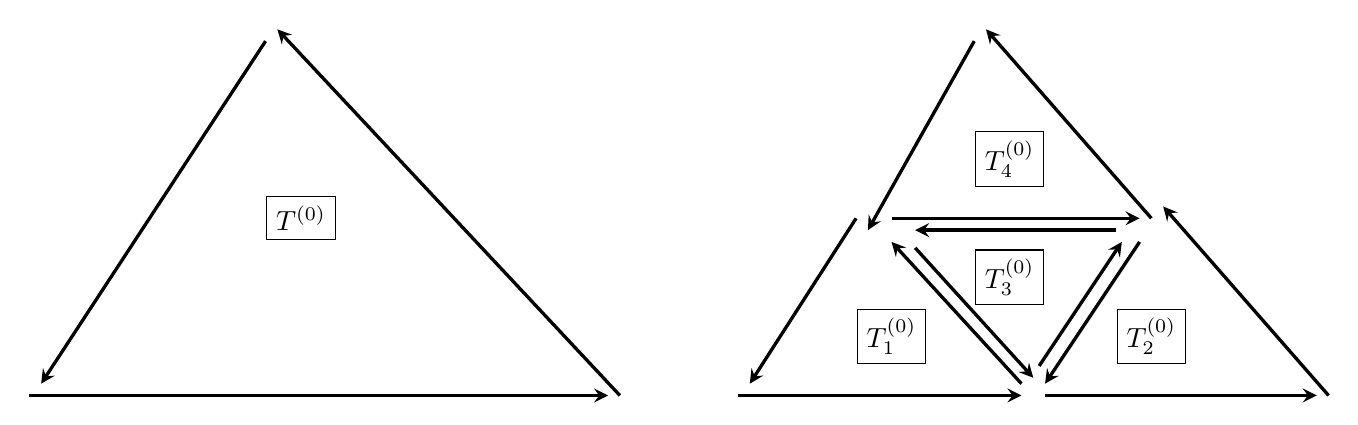
\begin{tikzpicture}[scale = 1.5]
            \tikzstyle{arrow} = [very thick,->,>=stealth]
            \draw [arrow] (0, 0) -- (4.9, 0);
            \draw [arrow] (5, 0) -- (2.1, 3.1);
            \draw [arrow] (2, 3) -- (0.1, 0.1);

            \draw [arrow] (6, 0) -- (8.4, 0);
            \draw [arrow] (8.6, 0) -- (10.9, 0);

            \draw [arrow] (11, 0) -- (9.6, 1.6);
            \draw [arrow] (9.5, 1.5) -- (8.1, 3.1);

            \draw [arrow] (8, 3) -- (7.1, 1.4);
            \draw [arrow] (7, 1.5) -- (6.1, 0.1);

            \draw [arrow] (7.3, 1.5) -- (9.4, 1.5);
            \draw [arrow] (8.4, 0.1) -- (7.3, 1.3);
            \draw [arrow] (9.4, 1.3) -- (8.6, 0.1);

            \draw [arrow] (9.2, 1.4) -- (7.5, 1.4);
            \draw [arrow] (7.5, 1.25) -- (8.5, 0.15);
            \draw [arrow] (8.55, 0.25) -- (9.25, 1.3);

            \node[draw] at (2.3, 1.5) {$T^{(0)}$};
            \node[draw] at (7.3, 0.5) {$T_1^{(0)}$};
            \node[draw] at (9.5, 0.5) {$T_2^{(0)}$};
            \node[draw] at (8.3, 1) {$T_3^{(0)}$};
            \node[draw] at (8.3, 2) {$T_4^{(0)}$};
            
        \end{tikzpicture}    
    \end{figure}
    
    We divide the original triangle into smaller triangles and choose their orientations in a way so that these cancel each other and only the orientation of the original big triangle remains.

    Then;

    $$\int_{T^{(0)}} f(z)dz = \int_{T_1^{(1)}} f(z)dz + \int_{T_2^{(1)}} f(z)dz + \int_{T_3^{(1)}} f(z)dz + \int_{T_4^{(1)}} f(z)dz$$

    So, there exist $j$ such that; 

    $$\left\vert  \int_{T^{(0)}} f(z)dz \right\vert \leq 4 \left\vert \int_{T_j^{(1)}} f(z)dz \right\vert $$

    We choose this $T_j^{(1)}$ and rename it as $T^{(1)}$ and similarly as before define its diameter and perimeter as $d^{(1)}$ and $p^{(1)}$. Continuing in this way, we obtain a sequence of smaller triangles, $T^{(n)}$, and in general;

    $$d^{(n)} = \dfrac{d^{(0)}}{2^n} \qquad p^{(n)} = \dfrac{p^{(0)}}{2^n}$$
    
    and also,

    $$\left\vert  \int_{T^{(0)}} f(z)dz \right\vert \leq 4^n \left\vert \int_{T^{(n)}} f(z)dz \right\vert $$

    Denoting the solid triangle or the compact set bounded by $T^{(n)}$ as $\mathcal{T}^{(n)}$, we obtain a sequence of compact sets whose diameter goes to $0$. By Cantor Intersection Theorem, we hence have existence of a point $z_0$ such that, $z_0$ lies inside each of the triangle. 
    
    Since, $f$ is analytic at $z_0$, 
    $$f(z) = f(z_0) + f'(z_0) (z- z_0) + \psi(z) (z - z_0)$$

    by a Taylor series expansion, where $\psi(z) \rightarrow 0$ as $z \rightarrow z_0$. However, the first two terms of the series have primitives and hence integrating them over the curves $T^{(n)}$ would yield $0$ for both these functions.

    Therefore,

    \begin{align*}
        \int_{T^{(n)}} f(z)dz 
        & = \int_{T^{(n)}} \psi(z) (z - z_0) dz\\
        & \leq \vert \sup_{z \in \mathcal{T}^{(n)} }\psi(z) \vert \int_{T^{(n)}} (z - z_0) dz\\
        & \leq \epsilon_n d^{(n)} p^{(n)}\\
        & \leq \dfrac{1}{4^n}\epsilon_n d^{(0)} p^{(0)}\\
    \end{align*}

    where $\epsilon_n \rightarrow 0$ as $n \rightarrow \infty$. However,

    $$\left\vert \int_{T} f(z)dz \right\vert < 4^n \left\vert \int_{T^{(n)}} f(z)dz \right\vert  \leq \epsilon_n d^{(0)} p^{(0)} \rightarrow 0$$

    which completes the proof.
\end{proof}

A simple corollary is as follows:

\begin{corollary}
    If $f$ is analytic in an open set that contains a rectangle $R$, and the area enclosed by it, then $\int_R f(z)dz = 0$.
\end{corollary}

\begin{proof}
    The proof follows immediately from the previous theorem once you break the rectangle into two triangles with opposite orientation.

    \begin{figure}[ht]
        \centering
        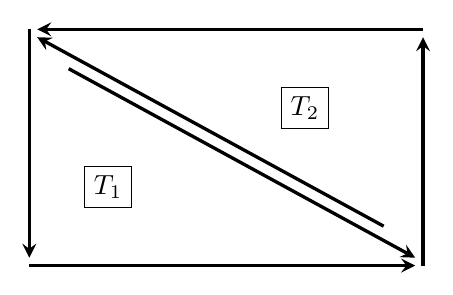
\begin{tikzpicture}
            \tikzstyle{arrow} = [very thick,->,>=stealth]
            
            \draw [arrow] (0, 0) -- (4.9, 0);
            \draw [arrow] (5, 0) -- (5, 2.9);
            \draw [arrow] (5, 3) -- (0.1, 3);
            \draw [arrow] (0, 3) -- (0, 0.1);
            
            \draw [arrow] (4.5, 0.5) -- (0.1, 2.9);
            \draw [arrow] (0.5, 2.5) -- (4.9, 0.1);
            
            \node[draw] at (1, 1) {$T_1$};
            \node[draw] at (3.5, 2) {$T_2$};
        \end{tikzpicture}
    \end{figure}
\end{proof}


% CLASS 8 FROM HERE

\begin{proposition}
    An analytic function $f$ in an open disc $D$ has a primitive in that disc.
\end{proposition}

\begin{proof}
    We may assume without the loss of generality that the center of the disc $D$ is $0$, the origin, otherwise we can simply apply the same argument after translation of the origin.

    Given, $z \in D$, consider the piecewise smooth curve $\gamma_z$ which consists of two segments.
    \begin{enumerate}
        \item First segment joins $0$ and $\Re z = \tilde{z}$ by moving in the horizontal direction.
        \item Second segment joins $\tilde{z} = \Re z$ to $z$ by moving in the vertical direction.
    \end{enumerate}

    Define, $F(z) = \int_{\gamma_z} f(w)dw$, here, the choice of the curve $\gamma_z$ gives an unambiguous definition to the function $F(z)$.

    Our claim is that $F$ is analytic in $D$ and $F'(z) = f(z)$, i.e. $F$ is precisely the primitive that we are looking for.

    To see this, consider $z \in D$ and choose $h$ such that $(z + h) \in D$, then;

    $$F(z + h) - F(z) = \int_{\gamma_{z+h}} f(w)dw - \int_{\gamma_{z}} f(w)dw = \int_{\eta} f(w)dw$$

    where $\eta$ is the straight line segment joining $z$ and $(z + h)$. Also, as $f$ is analytic in $D$, it is continuous in $D$, particularly at $z$. 

    Therefore, $f(w) = f(z) + \psi(w)$, where $\psi(w) \rightarrow 0$ as $w \rightarrow z$. Hence, we finally obtain;

    \begin{align*}
        F(z+h) - F(z)
        & = \int_{\eta} \left[ f(z) + \psi(w) \right]dw\\
        & = f(z) \int_{\eta} dw + \int_{\eta} \psi(w)dw\\
        & \leq f(z) (z + h - h) + \sup_{w \in \eta} \vert \psi(w) \vert L(\eta)\\
        & = f(z) h +  \sup_{w \in \eta} \vert \psi(w) \vert \vert h\vert
    \end{align*}

    Hence,

    $$\dfrac{F(z + h) - F(z)}{h} = f(z) + \lim_{h \rightarrow 0}\sup_{w \in \eta} \vert \psi(w) \vert = f(z)$$

    which completes the proof.
\end{proof}

\begin{note}
    Note that, the disc $D$ does not have any special property attached to it except that the curve $\gamma_z$ lies entirely in $D$.
\end{note}

\begin{theorem}[Cauchy's Theorem for a disc]
    If $f$ is analytic in a disc $D$ and $\gamma$ is a closed curve in $D$, then $\int_{\gamma} f(z)dz = 0$.
\end{theorem}

\begin{proof}
    By using the previous proposition, it follows that $f$ has a primitive in $D$, and by using \cref{cor:weak-cauchy}, the rest follows.
\end{proof}

\begin{corollary}
    Suppose, $f$ is analytic in an open set $\Omega$ containing the circle $C$ and the region enclosed by it. Then, $\int_{C} f(z)dz = 0$.
\end{corollary}

\begin{proof}
    Let, $D$ be the disc such that, its boundary $\partial D = C$. Then, there exists a slightly larger disc $D' \supset D$ such that, $f$ is analytic on $D'$. Applying Cauchy's thoerem on this $D'$ yields the result.

    \begin{note}
        To show the existence of the larger circle $D'$, let us assume that $C$ represents a circle with center at the origin. Let, $C = \left\{ z : z = r e^{i\theta} \right\}$.

        Now, any point $r e^{i\theta}$ is an interior point of $\Omega$. It is enough to show that, there exists $\epsilon > 0$, such that $s e^{i\theta} \in \Omega$ for all $s \in (r - \epsilon, r + \epsilon)$, $\theta \in \R$.

        Suppose it is not. Then, for every $n \in \N$, there exists $z_n = s_n e^{i\theta_n}$ such that $s_n \notin (r - 1/n, r + 1/n)$. Now, since $\left\{z_n\right\}$ is a bounded sequence, there exists a convergent subsequence, $z_{n_k} \rightarrow z_0$, which would imply $\vert z_0 \vert = r$, i.e. $z_0 = r e^{i\theta_0} \in C$ for some $\theta_0 \in \R$. 
        
        However, $\Omega$ being an open set, there exists $B_{\delta}(z_0)$ contianed inside the set $\Omega$ and containing points from $z_{n_k}$, which leads to a contradiction as all points of $z_n$'s are chosen in a way to not belong to $\Omega$.
    \end{note}
\end{proof}

It should be noted that a construction similar to the one proving existence of primitive of a function analytic in a disc holds for any curve where the notion of region bounded by the curve is unambiguous; and it is possible to orient the curve such that the area enclosed by it lies to the left as we traverse along the curve.

An important exmaple is the so called \textbf{Keyhold Contour} which is illustrated below:

\begin{figure}[h]
    \centering
    \includegraphics[width = 0.3\linewidth]{complex-figures/keyhole-contour.png}
\end{figure}

\begin{example}
    Here, $\Gamma$ denotes the curve and $\Gamma_0$ the region enclosed by it. Using the exact same argument as in the case of the circle we can find another (slightly larger) keyhole $\Lambda$ such that $\Lambda_0$ (the region enclosed by it) contains $\Gamma \cup \Gamma_0$.

    Now fix some $z_0 \in \Gamma_0$. For $z \in \Lambda_0$, let $\gamma_z$ be any curve joining $z_0$ and $z$, consisting of only finitely many horizontal and veritcal segments. 

    \begin{exercise}
        Check that it is possible to do so!
    \end{exercise}

    If $\eta_z$ is any other such curve, by the corollary of Goursat's theorem for rectangles, it follows that;

    $$\int_{\gamma_z} f(w) dw = \int_{\eta_z} f(w) dw$$

    Then we simply define $F(z) = \int_{\gamma_z} f(w)dw$, and arguing as in the case of the circle, $F$ is a primitive for $f$ in $\Lambda_0$ and hence $\int_{\gamma} f(z)dz = 0$.
\end{example}

\begin{theorem}
    Suppose, $f$ is analytic in an open set that contains the closure of a disc $D$. If $C$ denotes the boundary circle of this disc with positive orientation, then
    $$f(z) = \dfrac{1}{2\pi i} \int_{C} \dfrac{f(\xi)}{\xi - z} d\xi$$

    for any point $z \in D$.
\end{theorem}

\begin{proof}
    Fix $z \in D$ and consider the keyhole $\Gamma_{\delta, \epsilon}$ which avoids the point $z$. That means, the hole of the keyhole is centered at $z$, the radius of the circle around $z$ is $\epsilon$ and the width of the corridor is $\delta$ (i.e. the width of the straight segment).

    Note that, $F(\xi) = \dfrac{f(\xi)}{(\xi - z)}$ is analytic at every point except $z$. By Cauchy's theorem, $\int_{\Gamma_{\delta, \epsilon}} F(\xi)d\xi = 0$ for the chosen contour.

    Now, we make the corridor narrower by letting $\delta \rightarrow 0$ and use the continuity of $F$ to prove that in the limit, the integral over the two sides of the corridor cancels out. The remaining part consists of two curves, the large boundary circle $C$ with a positive orientation and a small circle $C_{\epsilon}$ centered at $z$ (and radius $\epsilon$) with negative orientation.

    To see what happens to the integral over the small circle, we write;

    $$F(\xi) = \dfrac{f(\xi) - f(z)}{(\xi - z)} + \dfrac{f(z)}{(\xi - z)}$$

    Now, since $f$ is analytic, this means the first term on the RHS is bounded, so its integral over $C_\epsilon$ goes to zero as $\epsilon \rightarrow 0$.

    Next, note that,

    \begin{align*}
        \int_{C_\epsilon} \dfrac{f(z)}{(\xi - z)} d\xi 
        & = f(z) \int_{C_\epsilon} \dfrac{d\xi}{(\xi - z)}\\
        & = - f(z) \int_{0}^{2\pi} \dfrac{\epsilon i e^{-it} dt}{\epsilon e^{-it}} \qquad \text{ since } \xi = z + \epsilon e^{-it}\\
        & = - if(z) \int_{0}^{2\pi} dt\\
        & = -2\pi i f(z)
    \end{align*}
\end{proof}

\begin{remark}
    The theorem holds with circle $C$ replaced by rectangle $R$.
\end{remark}

\begin{corollary}
    If $f$ is analytic in an open set $\Omega$ then $f$ is infinitely many times complex differentiable in $\Omega$. Moreover, if $C$ is a circle such that the disc $D$ with boundary $C$ is also contained in $\Omega$, then;

    $$f^{(n)}(z) = \dfrac{n!}{2\pi i} \int_{C} \dfrac{f(\xi)}{(\xi - z)^{(n+1)}} d\xi \qquad \forall z \in D$$
\end{corollary}

\begin{proof}
    Note that for $n = 0$, we get back Cauchy's Integral formula. 
    So, we use induction on $n$.

    Suppose, $f$ is complex differentiable $(n-1)$ times and by the induction hypothesis,

    $$f^{(n-1)}(z) = \dfrac{(n-1)!}{2\pi i} \int_{C} \dfrac{f(\xi)}{(\xi - z)^n} d\xi$$

    Therefore,
    $$
    \dfrac{f^{(n-1)}(z + h) - f^{(n-1)}(z)}{h} 
    = \dfrac{(n-1)!}{2\pi i} \int_{C} \dfrac{f(\xi)}{h} \left[ \dfrac{1}{(\xi - z - h)^n} - \dfrac{1}{(\xi - z)^n} \right]d\xi
    $$

    Let us simplify the integrad;
    
    \begin{align*}
        & \left[ \dfrac{1}{(\xi - z - h)^n} - \dfrac{1}{(\xi - z)^n} \right]\\
        = \quad & \left[ \dfrac{1}{(\xi - z - h)} - \dfrac{1}{(\xi - z)} \right] \left[ \dfrac{1}{(\xi - z - h)^{n-1}} + \dfrac{1}{(\xi - z - h)^{n-2}}\dfrac{1}{(\xi - z)} + \dots + \dfrac{1}{(\xi - z)^{n-1}}  \right]\\
        = \quad & \dfrac{h}{(\xi - z - h)(\xi - z)} \left[ \dfrac{1}{(\xi - z - h)^{n-1}} + \dfrac{1}{(\xi - z - h)^{n-2}}\dfrac{1}{(\xi - z)} + \dots + \dfrac{1}{(\xi - z)^{n-1}}  \right]
    \end{align*}

    $$
    \therefore \lim_{h\rightarrow 0} \dfrac{f^{(n-1)}(z + h) - f^{(n-1)}(z)}{h} = \dfrac{(n-1)!}{2\pi i} \int_{C} \dfrac{f(\xi)}{(\xi - z)^2} \dfrac{n}{(\xi - z)^{(n-1)}} d\xi
    $$

    i.e.

    $$f^{(n)}(z) = \dfrac{n!}{2\pi i} \int_{C} \dfrac{f(\xi)}{(\xi - z)^{(n+1)}} d\xi$$

    This completes the inductive step.
\end{proof}

\begin{corollary}[Cauchy inequalities]
    If $f$ is analytic in an open set that contains the closure of a disc $D$ centered at $z_0$ and of radius $R$, then;
    $$\vert f^{(n)}(z_0) \vert \leq \dfrac{n! \Vert f\Vert_C}{R^n}$$
    where $C = \partial D$, and $\Vert f\Vert_C = \sup_{z \in C} \vert f(z) \vert$
\end{corollary}

\begin{proof}
    Applying Cauchy's integral formula for $f^{(n)}(z_0)$, we obtain;

    \begin{align*}
        \vert f^{(n)}(z_0) \vert 
        & = \vert \dfrac{n!}{2\pi i} \int_C \dfrac{f(\xi)}{(\xi - z_0)^{(n+1)}}d\xi \vert\\
        & = \dfrac{n!}{2\pi} \vert \int_{0}^{2\pi} \dfrac{f(z_0 + R e^{i\theta}) R i e^{i\theta}}{(Re^{i\theta})^{(n+1)}} d\theta \vert\\
        \leq \dfrac{n!}{2\pi} \dfrac{\Vert f \Vert_C}{R^n} 2\pi
        = \dfrac{n! \Vert f\Vert_C}{R^n}
    \end{align*}
\end{proof}


Perhaps the most important consequence of the Cauchy Integral Formula is the existence of power series expansion of an analytic function.

\begin{theorem}
    Suppose $f$ is analytic in an open set $\Omega$. If $D$ is a disc having center at $z_0$ whose closure is contained in $\Omega$, then $f$ has a power series expansion at $z_0$:
    $$f(z) = \sum_{n= 0}^{\infty} a_n (z - z_0)^n \qquad \forall z \in D$$
    where the coefficients are given by $a_n = \dfrac{f^{(n)}(z_0)}{n!}$ for all $n \geq 0$.
\end{theorem}

\begin{proof}
    Applying Cauchy's Integral Formula, we have for $z \in D$,

    $$f(z) = \dfrac{1}{2\pi i} \int_{C} \dfrac{f(\xi)}{(\xi - z)} d\xi$$

    where $C = \partial D$. Write $(\xi - z) = (\xi - z_0) - (z - z_0) = (\xi - z_0) \left[ 1 - \dfrac{z - z_0}{\xi - z_0} \right]$

    Note that, $\xi \in C$, and $z \in D$, therefore, $\left\vert \dfrac{z - z_0}{\xi - z_0} \right\vert < r$ for some $0 < r < 1$.

    $$\dfrac{1}{(\xi - z)} = \dfrac{1}{(\xi - z_0)} \dfrac{1}{1 - \dfrac{z - z_0}{\xi - z_0}} = \dfrac{1}{(\xi - z_0)} \sum_{n = 0}^{\infty} \left( \dfrac{z - z_0}{\xi - z_0} \right)^n$$, the convergence of the above geometric series being uniform. This enables us to interchange the infinite sum with the integral $i$ and hence,

    $$f(z) = \sum_{n = 0}^{\infty} \left( \dfrac{1}{2\pi i} \int_{C} \dfrac{f(\xi)}{(\xi - z_0)^{(n+1)}}d\xi \right) (z - z_0)^{n}$$

    This proves that $f$ has a power series expansion and the formula for the coefficients is obtained by comparing with the formula for the derivative in the Cauchy's Integral formula.
\end{proof}

\begin{note}
    A power series defines an infinitely complex differentiable function in its disc of convergence, thus the theorem gives an alternative proof that an analytic function is infinitely many times complex differentiable.

    Recall that $f$ is said to the ``entire'' if it is analytic everywhere. Therefore, an analytic function has a power series expansion around any point, say $0$, that converges in all of $\C$.
\end{note}


\subsection{Liouville's Theorem and Applications}

\begin{theorem}[Liouville's Theorem]
    Any bounded entire function is constant.
\end{theorem}

\begin{proof}
    We will show $f' \equiv 0$. That would imply $f$ is constant.

    For each $z_0 \in \C$, and $R > 0$, from the Cauchy's inequality we get;

    $$\vert f'(z_0)\vert \leq \dfrac{\Vert f\Vert_{B_R(z_0)}}{R}$$

    Letting $R \rightarrow 0$, we get $\vert f'(z_0) \vert = 0$.
\end{proof}

Some applications of Liouville's theorem are as follows.

\begin{theorem}[Fundamental Theorem of Algebra]
    Every non constant polynomial $P(z) = a_nz^n + \dots + a_1 z + a_0$, where $a_i \in \C$, for all $0 \leq i \leq n$, has a root in $\C$.
\end{theorem}

\begin{proof}
    Suppose not. Then, $\dfrac{1}{P(z)}$ is an entire function.

    We shall show that $\dfrac{1}{P(z)}$ is bounded. For this, note that;

    $$
    \dfrac{P(z)}{z^n} = a_n + \left( \dfrac{a_{n-1}}{z} + \dots + \dfrac{a_1}{z^{n-1}} + \dfrac{a_0}{z^n}\right) \qquad \forall z \neq 0
    $$

    Assume $a_n \neq 0$, then the above quantity converges to $a_n$ as $\vert z \vert \rightarrow \infty$. Therefore, there exists some $R$ such that,

    $$\left\vert \dfrac{P(z)}{z^n} \right\vert \geq \dfrac{\vert a_n \vert}{2} \qquad \forall \vert z \vert > R$$

    i.e. $P$ is bounded below for $\vert z \vert > R$. Now, we assumed that $P$ has no roots in the disc $\vert z \vert \leq R$. Moreover, $P$ is continuous, hence $P$ is bounded below in the disc as well. This implies that, $\dfrac{1}{P(z)}$ is bounded.

    Now, an application of Liouville's theorem shows that $\dfrac{1}{P(z)}$ must be a constant function, hence $P(z)$ must be constant. This is a contradiction as $P$ is given to be a non-constant polynomial.
\end{proof}

\begin{remark}
    Using induction on the degree of $P$, say equal to $n$, we can conclude that $P$ has exactly $n$ roots in $\C$. If these roots are denoted by $\alpha_1, \alpha_2, \dots \alpha_n$, then $P$ can be factorized as;

    $P(z) = a_n (z - \alpha_1)(z - \alpha_2)\dots (z - \alpha_n)$
\end{remark}

The following theorem captures the behavior of the zeros of an analytic function in a connected open set $\Omega$.

\begin{theorem}
    Suppose, $f$ is analytic on a connected open set $\Omega$ and the zeroes of $f$ are a sequence of distinct points having a limit point in $\Omega$. Then $f$ is identically zero.
\end{theorem}

\begin{proof}
    Suppose, $\left\{ w_k \right\}_{k=1}^{\infty} \subset Z(f) = \left\{ z\in\C : f(z) = 0\right\}$ and $z_0 \in \Omega$ is a limit point of this sequence.

    \begin{result}
        $f \equiv 0$ in a small neighbourhood of $z_0$. 
    \end{result}

    To see this, consider a disc $D$ with center $z_0$ such that $D \subset \Omega$ and consider the power series expansion of $f$ in $D$, i.e.

    $$f(z) = \sum_{n=0}^{\infty} a_n (z - z_0)^n$$

    If $f$ is not identically equal to $0$, then there exist $m$ such that $a_m \neq 0$. Take the smallest such $m$.

    Then, $f(z) = a_m(z - z_0)^m \left[ 1  + g(z - z_0) \right]$

    where $g(z - z_0) \rightarrow 0$ as $z \rightarrow z_0$, due to higher powers in the power series. Putting $z = w_k$, we get that RHS becomes $a_m(w_k - z_0)^m \left[ 1 + g(w_k - z_0) \right]$, which is not equal to $0$, but the LHS $f(w_k) = 0$. This leads to a contradiction, which proves the claim (or the result).

    Now, we consider $U = (Z(f))^\circ$, which is non-empty and open set by the claim. Take, $z_n \in U$, such that $z_n \rightarrow z$. Then, $f(z) = \lim_{n} f(z_n) = 0$, by continuity.

    Again, by the claim, $z$ is an interior point of $Z(f)$, then $z \in U$. This says that $U$ must be closed as well. Let, $V = U^c$. Then, clearly, $U$ and $V$ are non-empty disjoint open sets, contradiction to the fact that $\Omega$ is connected. Hence, $U = \Omega$, which implies $f(z) = 0 \quad \forall z \in \Omega$.

\end{proof}

\begin{corollary}
    Suppose, $f$ and $g$ are two analytic functions that match on some non-empty open subset of $\Omega$ (or more generally, on a sequence of distinct points with limit point in $\Omega$). Then, $f(z) = g(z)$ for any $z \in \Omega$. 
\end{corollary}


\begin{theorem}[Morera's theoem]
    Let, $f : \Omega \rightarrow \C$, is continuous in its domain $\Omega$. It is given that $\int_T f(z)dz = 0$ for all triangles $T$ such that the triangle $T$ and the area enclosed by it lie completely inside $\Omega$.
    Then, $f$ is analytic.    
\end{theorem}

\begin{proof}
    Take any $z_0 \in \Omega$ such that there exists some $r > 0$ such that $B_r(z_0) \subseteq \Omega$. 

    For any $z \in B_r(z_0)$, define $F(z) = \int_{[z_0, z]} f(u)du$, where $[z_0, z]$ denotes the straight line segment joining $z_0$ and $z$. Consider the triangle $T$ given by the vertices $z_0, z$ and $(z + h)$, then by the given condition (assume $(z + h) \in B_r(z_0)$), we get;
    
    $$0 = \int_T f(z)dz = \int_{[z_0, z]} f(u)du + \int_{[z, z+h]}f(u)du + \int_{[z+h, z_0]}f(u)du$$

    Therefore,
    \begin{align*}
        \left\vert \dfrac{F(z+h) - F(z)}{h} - f(z) \right\vert
        & = \left\vert \dfrac{1}{h}\int_{[z, z+h]} f(u)du  - f(z)\right\vert \\
        & = \left\vert \dfrac{1}{h}\int_{[z, z+h]} (f(u) - f(z)) du \right\vert\\
    \end{align*}

    By continuity of $f$, given any $\epsilon > 0$, there exists $\delta > 0$, such that $\vert u - z\vert < \delta$, then $\vert f(u) - f(z) \vert < \epsilon$. Hence, if $\vert h \vert < \delta$, we have;

    \begin{align*}
        \left\vert \dfrac{F(z+h) - F(z)}{h} - f(z) \right\vert 
        & \leq \vert \dfrac{\epsilon \vert h\vert }{h}\vert \\
        & = \epsilon
    \end{align*}

    Since $\epsilon$ is arbitrary, $\left\vert \dfrac{F(z+h) - F(z)}{h} - f(z) \right\vert \rightarrow 0$ as $\vert h \vert \rightarrow 0$, thus showing $F'(z) = f(z)$, i.e. $F$ is analytic in $\Omega$. Hence, $f$, being the derivative of $F$ must also be analytic in $\Omega$.
\end{proof}

% Q & A Section
\subsection{Example Problems}

\begin{exercise}
    Suppose, $C$ is the circle enclosing the point $(2, 0)$. What is $\int_{C} \dfrac{e^{z^2}}{(z - 2)}dz$?
\end{exercise}

\begin{figure}[h]
    \centering
    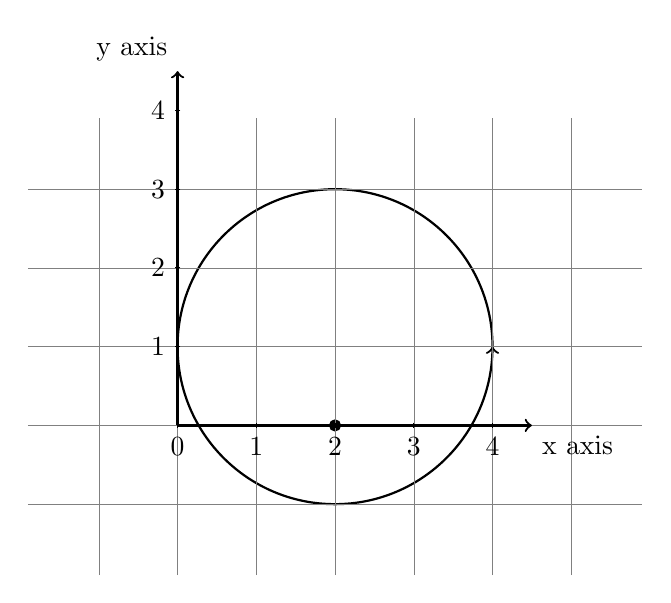
\begin{tikzpicture}
        \draw[
            thick,
            decoration={markings, mark=at position 1 with {\arrow{>}}},
            postaction={decorate}
            ]
            (2,1) circle (2);
        \filldraw [black] (2,0) circle (2pt);
        \draw[step=1cm,gray,very thin] (-1.9,-1.9) grid (5.9,3.9);
        \draw[thick,->] (0,0) -- (4.5,0) node[anchor=north west] {x axis};
        \draw[thick,->] (0,0) -- (0,4.5) node[anchor=south east] {y axis};
        \foreach \x in {0,1,2,3,4}
            \draw (\x cm,1pt) -- (\x cm,-1pt) node[anchor=north] {$\x$};
        \foreach \y in {1,2,3,4}
            \draw (1pt,\y cm) -- (-1pt,\y cm) node[anchor=east] {$\y$};
    \end{tikzpicture}    
\end{figure}


Let, $f(z) = e^{z^2}$, which is an entire function. $C$ is given in counterclockwise orientation. Given any point $w$ inside the disc bounded by $C$,

$$f(w) = \dfrac{1}{2\pi i} \int_C \dfrac{f(w)}{(z - w)}dz$$

We can evaluate the above integral if we plug if $w = 2$, 

$$\therefore \qquad f(2) = \dfrac{1}{2\pi i} \int_C \dfrac{e^{z^2}}{(z - 2)}dz$$

Hence, $\int_{C} \dfrac{e^{z^2}}{(z - 2)} = 2\pi i f(2) = 2\pi i e^{2^2} = 2\pi i e^{4}$.

\begin{exercise}
    Evaluate the same integral as in the previous problem, but this time, over a circle that does not enclose the point $(2, 0)$.
\end{exercise}

In this case, let $f(z) = \dfrac{e^{z^2}}{(z - 2)}$, analytic in the region closed by $C$. By Cauchy's theorem, $\int_C f(z)dz = 0$.


\begin{exercise}
    Evaluate $\int_C \dfrac{e^{2z}}{z^4}dz$, where $C$ is the unit circle.
\end{exercise}

Let, $f(z) = e^{2z}$. Since, $0 \in D$, the unit disc, it is clear that the integrand itself is not analytic in $C$. However,

$$f'''(0) = \dfrac{3!}{2\pi i} \int_C \dfrac{e^{2z}}{(z - 0)^4}dz$$

and therefore,

$$\int_C \dfrac{e^{2z}}{z^4}dz = \dfrac{2\pi i}{6} f'''(0) = \dfrac{8\pi i}{3}$$

since, $f'''(z) = 8e^{2z}$.


\begin{exercise}
    Compute $\int_\gamma \dfrac{\cos z}{z(z^2 + 4)}dz$ where $\gamma$ is the rectangular contour shown in the figure.
\end{exercise}

\begin{figure}[h]
    \centering
    \begin{tikzpicture}
        \draw[step=1cm,gray,very thin] (-2.9,-2.9) grid (2.9,2.9);
        \draw[thick,->] (-3.5,0) -- (3.5,0) node[anchor=north west] {x axis};
        \draw[thick,->] (0,-3.5) -- (0,3.5) node[anchor=south east] {y axis};        
        \draw[ultra thick, ->, dashed, red] (1, -1.5) -- (1, 1.5);
        \draw[ultra thick, ->, dashed, red] (1, 1.5) -- (-1, 1.5);
        \draw[ultra thick, ->, dashed, red] (-1, 1.5) -- (-1, -1.5);
        \draw[ultra thick, ->, dashed, red] (-1, -1.5) -- (1, -1.5);
        \filldraw (0,2) circle[radius=1.5pt];
        \node[right=4pt of {(0,2)}, outer sep=2pt,fill=white] {$2i$};
        \filldraw (0,-2) circle[radius=1.5pt];
        \node[right=4pt of {(0,-2)}, outer sep=2pt,fill=white] {$-2i$};   
    \end{tikzpicture}
\end{figure}

Let, $f(z) = \dfrac{\cos z}{(z^2 + 4)}$

Clearly, $f$ is analytic in the region enclosed by $\gamma$, since the roots of $(z^2 + 4)$, i.e. $z = \pm 2i$ lies outside the region enclosed by $\gamma$. So, the integral can be rewritten as;

$$
\int_C \dfrac{f(z)}{z}dz = 2\pi i f(0) = 2\pi i \dfrac{1}{4} = \dfrac{\pi i}{2}
$$

\begin{exercise}
    Find $\int_C \dfrac{dz}{(z^2 + 4)^2}$, where $C$ is the circle such that, it is centered at $i$ and have a radius more than 1 but less than 2. In other words, the circle encloses the points $i, 2i$ but not $(-i)$ or $(-2i)$.
\end{exercise}

For this problem, we factorize the denominator as;

$$
(z^2 + 4)^2 = (z - 2i)^2 (z + 2i)^2
$$

Since, the circle encompasses $2i$, but not $(-2i)$, we need to remove $(z - 2i)$ from consideration when building the function. So, $f(z) = \dfrac{1}{(z + 2i)^2}$. 

Now, by Cauchy's formula for derivatives;

$$
\int_{C} \dfrac{dz}{(z^2 + 4)^2} = \int_C \dfrac{f(z)dz}{(z - 2i)^2} = 2\pi i f'(2i) = 2\pi i \left[ \dfrac{-2}{(z + 2i)^3} \right]_{z = 2i} = \dfrac{\pi}{16}
$$

\begin{exercise}
    $\int_C \dfrac{z}{(z^2 + 4)}dz$ over the circle $C$ centered at $0$ and with radius more than $2$.
\end{exercise}

Here, the integral has singularities at both $z = \pm 2i$, both of which are enclosed by the curve $C$. So, we need to use partial fractions.

Using partial fractions, we have 

$$\dfrac{z}{(z - 2i)(z + 2i)} = \dfrac{1/2}{(z - 2i)} + \dfrac{1/2}{(z + 2i)}$$

Therefore,

\begin{align*}
    \int_C \dfrac{z}{(z^2+ 4)}dz
    & = \dfrac{1}{2} \int_C \dfrac{dz}{(z - 2i)} + \dfrac{1}{2} \int_C \dfrac{dz}{(z + 2i)}\\
    & = \pi i + \pi i \qquad \text{as, } f(z) = 1 \text{ gives, } \dfrac{1}{2\pi i} \int_C \dfrac{dz}{(z - 2i)} = 1\\
    & = 2\pi i
\end{align*}


\begin{exercise}
    Compute the real integral,
    $$I = \int_{-\infty}^{\infty} \dfrac{1}{(x^2 + 1)^2} dx$$
\end{exercise}

Let us consider the half-circle with counterclockwise orientation lying above $x$-axis, with its curved side denoted as $C_R$ and its side on the part of the $x$-axis as $C_0$. Assume the circle is centered at the origin with a radius $R$, larger than 1, hence the half circle encompasses the point $i$.

We shall integrate, $f(z) = \dfrac{1}{(z^2 + 1)^2}$ over the closed contour $C_0 \cup C_R$. Note that, this $f(z)$ has only one singularity, namely $z = i$. Let, $g(z) = \dfrac{1}{(z + i)^2}$. Then, $g$ is analytic in the region enclosed by $\gamma = C_0 \cup C_R$. Then,

$$
\int_{\gamma} f(z)dz = \int_{C_0 \cup C_R} \dfrac{g(z)}{(z - i)^2}dz = 2\pi i g'(i) = 2\pi i \left[ \dfrac{-2}{(z + i)^3} \right]_{z = i} = \dfrac{-4\pi i}{(2i)^3} = \dfrac{\pi}{2}
$$

To evaluate $\int_{C_0} f(z)dz$ we parametrize $C_0$ by $\gamma(t) =t$, for $(-R) \leq t \leq R$, hence, as $R \rightarrow \infty$,

$$\int_{C_0} f(z)dz = \int_{-R}^{R} \dfrac{dx}{(x^2 + 1)^2} \rightarrow I$$

To evaluate $\int_{C_R} f(z)dz$, we parametrize $C_R$ as $\gamma(\theta) = Re^{i\theta}$, for $0 \leq \theta \leq \pi$. Then,

$$
\int_{C_R} f(z)dz = \int_{0}^{\pi} \dfrac{1}{(R^2 e^{2i\theta} + 1)^2} iRe^{i\theta}d\theta
$$

Now, $\vert R^2 e^{2i\theta} + 1\vert \geq \vert R^2 e^{2i\theta} \vert - 1 = (R^2 - 1)$. Hence,

\begin{align*}
    \left\vert \int_{C_R} f(z)dz \right\vert
    & \leq \int_{0}^{\pi} \left\vert \dfrac{iRe^{i\theta}}{(R^2 e^{2i\theta} + 1)^2}  \right\vert d\theta\\
    & \leq \int_{0}^{\pi} \dfrac{R}{(R^2 - 1)^2} d\theta\\
    & \dfrac{R}{(R^2 - 1)^2} \pi \rightarrow 0 \qquad \text{as, } R\rightarrow \infty
\end{align*}

On the other hand, $\int_\gamma f(z)dz = \pi/2$ for any $R > 1$. Therefore, $I = \pi/2$.

\begin{exercise}
    Show that, $\int_0^{\infty} \dfrac{(1 - \cos x)}{x^2} dx = \dfrac{\pi}{2}$
\end{exercise}

Here again, consider the function $f(z) = \dfrac{(1 - e^{iz})}{z^2}$ and integrate over the following curve;

\begin{figure}[h]
    \centering
    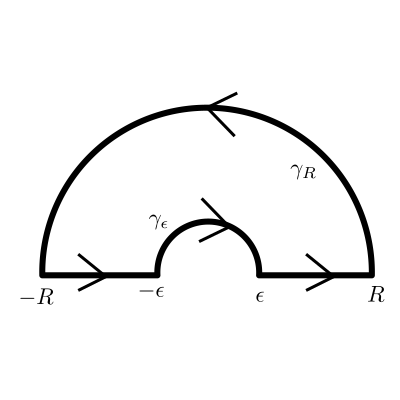
\includegraphics[width = 0.5\linewidth]{complex-figures/problem-8.png}
\end{figure}

where $\gamma_R$ and $\gamma_\epsilon$ are semicircles of radii $R$ and $\epsilon$ respectively, with the orientations as shown in the figure.

Cacuhy's theorem yields;

$$
\int_{-R}^{-\epsilon} \dfrac{(1 - e^{ix})}{x^2}dx + \int_{\gamma_\epsilon} \dfrac{(1 - e^{iz})}{z^2} dz + \int_{\epsilon}^{R} \dfrac{(1 - e^{ix})}{x^2} + \int_{\gamma_R} \dfrac{(1 - e^{iz})}{z^2} dz = 0$$

Now, $\left\vert \dfrac{(1 - e^{iz})}{z^2} \right\vert \leq \dfrac{2}{\vert z \vert^2}$. Therefore,

$$
\left\vert \int_{\gamma_R} \dfrac{(1 - e^{iz})}{z^2}dz \right\vert
\leq \int_{\gamma_R} \dfrac{2}{\vert z \vert^2} dz \leq \sup_{z \in \gamma_R} \dfrac{2}{\vert z \vert^2} L(\gamma_R) = \dfrac{2}{R^2} \pi R = \dfrac{2\pi}{R}
$$

From the above, we get; $\int_{\vert x \vert > \epsilon}\dfrac{(1 - e^{ix})}{x^2}dx = - \int_{\gamma_\epsilon} \dfrac{(1 - e^{iz})}{z^2} dz$. Now, $e^{iz} = 1 + iz - \dfrac{z^2}{2} - \dfrac{iz^3}{3!} + \dots$. So,

$$
\dfrac{(1 - e^{iz})}{z^2} = \dfrac{-iz}{z^2} + E(z)
$$

where $E(z)$ is bounded as $z \rightarrow 0$. Whereas, on $\gamma_\epsilon$, we have $z = \epsilon e^{i\theta}$, so, $dz = i\epsilon e^{i\theta} d\theta$, and hence;

$$
\int_{\gamma_\epsilon} \dfrac{(1 - e^{iz})}{z^2} dz \rightarrow \int_{\pi}^{0} \dfrac{-i\cdot i\epsilon e^{i\theta}}{\epsilon e^{i\theta}} d\theta = -\pi \quad \text{, as } \epsilon \rightarrow 0
$$

Taking real parts thus yields;

$$\int_{-\infty}^{\infty} \dfrac{(1 - \cos x)}{x^2}dx = \pi$$

and since the integrand is an even function, $\int_{0}^{\infty} \dfrac{(1 - \cos x)}{x^2}dx = \dfrac{\pi}{2}$.


\section{Sequence of Analytic Functions}
\subsection{Uniform Convergence on Compact Sets}

\begin{theorem}
    If $\left\{ f_n\right\}_{n = 1}^{\infty}$ is a sequence of analytic functions that converges uniformly to a function $f$ on every compact subset of $\Omega$. Then, $f$ is analytic in $\Omega$.

    We write this condition as $f_n \xrightarrow{UCC(\Omega)} f$.
\end{theorem}

\begin{proof}
    Suppose, $D$ is any disc such that, $\overline{D} \subseteq \Omega$ and let $T$ be any triangle in that disc. 

    Since, each $f_n$ is analytic, application of Goursat's theorem tells us $\int_T f_n(z)dz = 0$ for all $n \in \N$. Now, as $f_n \rightarrow f$ uniformly in $\overline{D}$, a compact set, so $f$ is continuous and $\int_T f_n(z)dz \rightarrow \int_T f(z)dz$. Therefore, $\int_T f(z)dz = 0$. Now, applying Morera's theorem, we get that $f$ is analytic in $D$. Since the conclusion holds for all $D$ such that $\overline{D} \subseteq \Omega$, $f$ must be analytic in $\Omega$.  
\end{proof}

\begin{note}
    This result is not true for real valued functions and real differentiablity. For example, every continuous function can be well approximated by polynomials, by using Weierstrass' theorem. While the polynomials are differentiable, any continuous function is not.
\end{note}

\begin{theorem}
    Assume, $f_n \xrightarrow{UCC(\Omega)} f$, and $f_n$'s are analytic in $\Omega$ (i.e. the assumptions of previous theorem holds), then $f_n' \xrightarrow{UCC(\Omega)} f$, i.e. the sequence of derivatives also converges uniformly to $f'$ on every compact subset of $\Omega$.
\end{theorem}

\begin{proof}
    Without loss of generality, assume $f_n \xrightarrow{UCC(\Omega)} 0$. We shall show that, $f_n' \xrightarrow{UCC(\Omega)} 0$.

    Let, $K \subseteq \Omega$, be a compact set. Since, $\Omega$ is open, for all $x \in K$, there exists $r_x > 0$ such that, $\left\{ z : \vert z - x \vert \leq r_x\right\} \subseteq \Omega$. 
    
    Now, consider the open cover $\cup_{x \in K} B_{r_x / 2}(x)$ of $K$. Since, $K$ is compact, there exists a finite subcover, i.e. there exists $x_1, x_2, \dots x_m \in K$ such that, $K \subseteq \cup_{i=1}^{m} B_{r_i/2}(x_i)$, where $r_i = r_{x_i}$ for all $i = 1, 2, \dots m$.

    \begin{note}
        Let, $F: \Omega \rightarrow \C$ be an analytic function. Then, for $z \in \Omega$, Cauchy's Integral Formula gives us, $F'(z) = \dfrac{1}{2\pi i} \int_\gamma \dfrac{F(w)}{(w - z)^2} dz$, where $\gamma$ is a bounding circle of radius $r$. Then,
        \begin{align*}
            \vert F'(z)\vert
            & = \dfrac{1}{2\pi} \left\vert \int_\gamma \dfrac{F(w)}{(z - w)^2} \right\vert\\
            & \leq \left\vert \sup_{\alpha \in \overline{B_r}} F(\alpha) \right\vert \dfrac{1}{2\pi} (2\pi r) \dfrac{1}{(r - \vert z \vert^2)}\\
            & = \left\vert \sup_{\alpha \in \overline{B_r}} F(\alpha) \right\vert \dfrac{r}{(r - \vert z \vert^2)}
        \end{align*}
    \end{note}

    Now, fix $i \in \left\{ 1, 2, \dots m\right\}$ and $\epsilon > 0$. Then, $\forall z \in \overline{B_{r_i/2}(x_i)} \subset B_{r_i}(x_i) \subset \overline{B_{r_i}(x_i)} \subset \Omega$,

    $$\vert f_n'(z) \vert \leq \dfrac{r_i}{(r_i / 2)^2} \sup_{w \in B_{r_i}(x_i)} f_n(w) < \epsilon \qquad \forall n > N_i$$

    because of uniform convergence of $f_n$'s. Thus, 

    $$\sup_{w \in B_{r_i/2}(x_i)} \vert f_n'(w) \vert < \epsilon \qquad \forall n > N_i$$

    Because the finite cover exists for $\Omega$, we can take $N = \max_{i = 1}^{m} N_i$, and then $\forall n > N$, the above holds and in other words, $f_n' \xrightarrow{UCC(\Omega)} 0$.
\end{proof}

\subsection{Classification of Singularities}

\begin{definition}
    \textbf{Isolated Singularity:} $f$ has an isolated singularity at $z = a$, if there exists $R > 0$ such that;
    \begin{enumerate}
        \item $f$ is defined
        \item and $f$ is analytic in $B_R(a) \backslash \left\{ a\right\}$, but not in $B_R(a)$.
    \end{enumerate}
\end{definition}

Isolated singularities are of three main types:

\begin{enumerate}
    \item Removable singularity.
    \item Pole.
    \item Essential singularity.
\end{enumerate}

\begin{definition}
    An isolated singularity of a function $f$ at a point $z = a$, is said to be a removable singularity if there exists an analytic function $g$ defined on some neighbourhood $B_R(a)$, i.e. $g : B_R(a) \rightarrow \C$ such that $f(z) = g(z)\qquad \forall z \neq a$.
\end{definition}

For example, $f(z) = \dfrac{\sin z}{z}$ has a removable discontinuity at $z = 0$. For a removable singularity of $f$ at a point $z = a$, the limit $\lim_{z \rightarrow a} f(z)$ exists.

\begin{theorem}
    If $f$ has an isolated singularity at the point $z = a$, then it is a removable singularity if and only if $\lim_{z \rightarrow a} (z - a)f(z) = 0$.
\end{theorem}

\begin{proof}
    If the point is a removable singularity, then clearly the limit $\lim_{z \rightarrow a} f(z)$ exists. But then, $\lim_{z \rightarrow a}(z - a) f(z) = \lim_{z\rightarrow a}(z - a) \lim_{z \rightarrow a} f(z) = 0$. 

    To show the converse, Suppose $f$ is analytic in $B_R(a) \backslash \left\{ a \right\}$, and define the function $g$ such that,

    $$
    g(z) = \begin{cases}
        (z - a) f(z) & \text{ if } z \neq a\\
        0 & \text{ if } z = a\\
    \end{cases}
    $$

   We are also given that the limit $\lim_{z \rightarrow a} (z-a)f(z) = 0 = \lim_{z \rightarrow a} g(z)$. Clearly, then $g$ is a continuous function. Now, it is enough to show that $g$ is analytic, as then $g(z) = (z - a)h(z)$, with $h(z)$ being another analytic function. However, $f$ and $h$ agree on all other points except $z = a$.

   To show $g$ is analytic, we shall apply Morera's theorem. Let, $T$ be a triangle in $B_R(a)$ and $\Delta$ be the solid triangle whose boundary is $T$. 

   If $a \notin \Delta$, then $\int_T g(z)dz = 0$, by Cauchy's theorem due to the fact that $f$ is analytic.

   If $a$ is a vertex of $T$, then consider the following construction. Choose, $x$ and $y$ on the sides of the triangle meeting at vertex $a$, close enough to the vertex $a$, and call that small triangle $T_1$. Also, make sure the orientation cancels out once you consider the triangle and the quadrilateral (two parts the bigger triangle $T$ is broken into). Since, $g$ is continuous and $g(a) = 0$, for any $\epsilon > 0$, $x$ and $y$ are chosen in such a way so that, $\vert g(z) \vert < \epsilon / L$ (where $L$ is the perimeter of $T$), for any $z$ in the small triangle $T_1$, formed by the vertices of $a, y, x$. Let, the quadrilateral be denoted as $P$, i.e. $P = \Delta(T) - \Delta(T_1)$. 

   Then, 

   $$\int_T g(z)dz = \int_{T_1} g(z)dz + \int_P g(z)dz = \int_{T_1} g(z)dz$$

   since, $\int_P g(z)dz = 0$, by Cauchy's theorem. However, 
   
   $$\left\vert \int_T g(z)dz \right\vert = \left\vert \int_{T_1} g(z)dz \right\vert \leq \sup_{z \in T_1} \vert g(z) \vert \times L < \epsilon$$

   Since, $\epsilon$ is arbitrary, this shows $\int_T g(z)dz = 0$, and thus by Morera's theorem, $g$ is analytic.

   If $a \in \Delta$, then we subdivide the original triangle into three triangles, such that they share $a$ as a common vertex. Then, the previous analysis applies to each of the triangle which completes the proof. 
\end{proof}

\begin{example}
    One example of pole is $f(z) = \dfrac{1}{z}$, then the function has a pole at $z = 0$. This means basically the function gets higher or lower as it approaches a certain point (i.e. the pole).
\end{example}

\begin{definition}
    An isolated singularity of a function $f$ at a point $a$ is said to be a pole if $\lim_{z \rightarrow a} \vert f(z) \vert = \infty$.
\end{definition}

Suppose, $f$ has a pole at the point $z = a$. Therefore, for all $M > 0$, there exists $\epsilon > 0$, such that $\vert f(z) \vert \geq M$, for all $0 < \vert z - a\vert < \epsilon$. Considering reciprocal, $\left\vert \dfrac{1}{f(z)} \right\vert \leq \dfrac{1}{M}$, and thus, $\lim_{z \rightarrow a} \vert \dfrac{1}{f(z)} \vert = 0$. Thus, applying the knowledge of the previous section, we see that the function $1/f$ has a removable singularity at $z = a$. Let, 

$$
h(z) = \begin{cases}
    \dfrac{1}{f(z)} & \text{ if } z \neq a\\
    0 & \text{ if } z= a\\
\end{cases}
$$

$h$ is analytic in $B_R(a)$ for some $R > 0$, thus, $h(z) = (z - a)^m h_1(z)$ for some analytic function $h_1$ with $h_1(a) \neq 0$ and some integer $m \geq 1$. Thus, $(z - a)^m f(z) = (h(z))^{-1}$ has a removable singularity at $z = a$. 

\begin{proposition}
    If $f$ is analytic in a domain $\Omega$ except for the point $z = a$, where it has a pole, then there exists a positive integer $m$ and an analytic function $g : \Omega \rightarrow \C$ such that, $f(z) = \dfrac{g(z)}{(z - a)^m}$.
\end{proposition}

\begin{definition}
    If $f$ has a pole at $z = a$ and $m$ is the smallest positive integer such that $(z - a)^m f(z)$ has a removable singularity at $z = a$, then $f$ is said to have a pole of order $m$ at $z = a$.
\end{definition}

\begin{note}
    If $m$ is the order of the pole at $z = a$, and $g$ is as mentioned above in the proposition, then $g(a) \neq 0$. In fact,

    \begin{align*}
        f(z)
        & = \dfrac{1}{(z - a)^m} g(z)\\
        & = \dfrac{1}{(z - a)^m} \left[ A_0 + A_1 (z - a) + \dots \right]\\
        & = \dfrac{B_{-m}}{(z - a)^m} + \dfrac{B_{-m+1}}{(z - a)^{m-1}} + \dfrac{B_{-1}}{(z - a)} + G(z)\\
    \end{align*}

    where $G(z)$ is analytic and the first part is called the principal part or singular part of $f$ at $z = a$.
\end{note}


% residue formula lecture
Let, the singular part is $P(z)$, and $C$ be any circle centered at $z_0$, then 

$$
\dfrac{1}{2\pi i} \int_C P(z)dz = B_{-1}
$$

where $B_{-1}$ is the coefficient of $(z - z_0)^{-1}$. 

\begin{definition}
    Suppose $f$ has a simple pole at $z_0$, then the residue of $f$ at $z_0$ is $\text{res}_{z_0}(f) = \lim_{z \rightarrow z_0}(z - z_0)f(z)$. In case $f$ has a pole of order $m$ at $z_0$, then 

    $$
    \text{res}_{z_0}(f) = \lim_{z \rightarrow z_0} \dfrac{1}{(m-1)!} \left(\dfrac{d}{dz}\right)^{(n-1)} \left[ (z - z_0)^m f(z) \right]
    $$    
\end{definition}

\begin{theorem}
    Suppose $f$ is analytic in an open set containing a circle $C$ (and the disc enclosed by it) except for a pole at $z_0$ inside $C$. Then,

    $$
    \int_C f(z)dz = 2\pi i \text{res}_{z_0}(f)
    $$
\end{theorem}

\begin{proof}
    Consider a keyhole contour $\gamma$ with the circle $C$ that avoids point $z_0$ with a keyhole circle of radius $\epsilon$ called $C_\epsilon$.

    Then by Cauchy's theorem, $\int_\gamma f(z)dz = 0$. The contribution due to the line segments of the corridor will cancel each other, and we obtain;

    $$
    \int_C f(z)dz = \int_{C_\epsilon} f(z)dz
    $$

    Now, applying Cacuhy's Integral formula to the constant function $a_{-1}$, we obtain;

    $$
    \dfrac{1}{2\pi i} \int_{C_\epsilon} \dfrac{a_{-1}}{(z - z_0)}dz = a_{-1}
    $$

    Similarly, 
    
    $$
    \dfrac{1}{2\pi i} \int_{C_\epsilon} \dfrac{a_{-k}}{(z - z_0)^k}dz = a_{-k} \qquad \forall k > 1
    $$

    by using the corresponding formula for derivatives. But in a neighbourhood of the point $z_0$, we can write;

    $$
    f(z) = \dfrac{a_{-n}}{(z - z_0)^n} + \dots + \dfrac{a_{-1}}{(z - z_0)} + G(z)
    $$

    By Cauchy's theorem, the integral $\int_{C_\epsilon}G(z) dz = 0$, hence $\int_{C_\epsilon} f(z)dz = a_{-1}$, which is same as the integral over $C$.
\end{proof}

The same result can be generalized if there is more than one poles.

\begin{corollary}
    Suppose $f$ is analytic in an open set containing a circle $C$ and its interior, except for poles at the point $z_1, z_2, \dots z_N$ inside $C$. Then,

    $$
    \int_C f(z)dz = 2\pi i \sum_{i=1}^{N} \text{res}_{z_k}(f)
    $$
\end{corollary}

\begin{proof}
    Consider a multiple keyhole contour with keyholes avoiding each of the $z_1, z_2, \dots z_N$, the poles, and apply the same logic to each of the keyholes.
\end{proof}

\begin{corollary}
    Suppose $f$ is analytic in an open set containing an arbitrary contour (and its interior), except for poles at $z_1, z_2, \dots z_N$ inside $\gamma$, then 

    $$
    \int_\gamma f(z)dz = 2\pi i \sum_{i=1}^{N} \text{res}_{z_k}(f)
    $$
\end{corollary}

This is called \textbf{Residue Formula}.


\begin{theorem}[Riemann's Theorem on removable singularities]
    Suppose $z_0 \in \Omega$ and $f : \Omega \backslash \left\{ z_0\right\} \rightarrow \C$ is a bounded analytic function, Then $z_0$ is a removable singularity of $f$.
\end{theorem}

\begin{proof}
    Since, $\Omega$ is an open set containing $z_0$, there must exists an open disc $D$ such that $z_0 \in D \subseteq \bar{D} \subseteq \Omega$, and let $C$ be the circle i.e. the boundary of $D$.

    We start by making a claim as follows:

    For $z \neq z_0 \in D$, $f(z) = \dfrac{1}{2\pi i} \int_C \dfrac{f(\xi)}{(\xi - z)}d\xi$.

    Once we assume this claim, the right hand side extendes to an analytic function to all of $D$, once we consider the parameteric substitution $\sigma(t) = z_0 + r e^{2\pi i t}$, with $0 < t < 1$. Note that the right hand side becomes,

    \begin{align*}
        \text{RHS}
        & = \dfrac{1}{2\pi i} \int_C \dfrac{f(\xi)}{(\xi - z)}d\xi\\
        & = \dfrac{1}{2\pi i} \int_{0}^{1} \dfrac{f(\sigma(t))}{(\sigma(t) - z)}\sigma'(t) dt\\
        & = \dfrac{1}{2\pi i} \int_{0}^{1} \dfrac{f(\sigma(t))}{(\sigma(t) - z)}r e^{2\pi i t} dt \\
        & = \dfrac{1}{2\pi i} \int_{0}^{1} F(z) \quad \text{where } F(z) \text{ is the integrand above}\\
        & = G(z)
    \end{align*}

    To see why $G(z)$ is analytic, note that,

    \begin{align*}
        \dfrac{G(z + h) - G(z)}{h} 
        & = \dfrac{1}{h} \int_{0}^{1} r f(\sigma(t)) e^{2\pi i t} \left[\dfrac{h}{(\sigma(t) - z - h)(\sigma(t) - z)} \right] dt\\
        & = \int_{0}^{1} r f(\sigma(t)) e^{2\pi i t} \left[\dfrac{1}{(\sigma(t) - z - h)(\sigma(t) - z)} \right] dt\\
        & \rightarrow \int_{0}^{1} r f(\sigma(t)) e^{2\pi i t} \left[\dfrac{1}{(\sigma(t) - z)^2} \right] dt \qquad \text{use Dominated Convergence Theorem here}
    \end{align*}

    Thus the right hand side becomes an analytic function, once we prove the claim.

    Fix $z \in D$ with $z \neq z_0$. Consider a multiple keyhole contour which avoids both the points $z_0$ and $z$ as centers of different keyholes. Consider the outside circle to have a positive orientation and then the inside circles would have a negative orientations. Let, $\epsilon$ be the radius of the inside circles (or keyholes) and the keyhole around $z_0$ is denoted by $\gamma_\epsilon'$ and the keyhole around $z$ is denoted by $\gamma_\epsilon$. The width of the narrow corridors goes to $0$.

    Similar to the proof of Cauchy's theorem, the contribution due to the two corridors cancel each other, hence in the limit we would have (by Cauchy's theorem),

    $$
    \int_C \dfrac{f(\xi)}{(\xi - z)} d\xi + \int_{\gamma_\epsilon}\dfrac{f(\xi)}{(\xi - z)} d\xi + \int_{\gamma_\epsilon'} \dfrac{f(\xi)}{(\xi - z)} d\xi = 0 
    $$

    Note that, exactly similar to the proof of Cauchy's integral formula,

    $$
    \int_{\gamma_\epsilon}\dfrac{f(\xi)}{(\xi - z)} d\xi = -2\pi i f(z)
    $$

    Using boundedness of the function $f$, we have for the final term,

    $$
    \left\vert \int_{\gamma_\epsilon'}\dfrac{f(\xi)}{(\xi - z)} d\xi \right\vert \leq C \times 2\pi \epsilon
    $$

    since, $f(\xi)$ is bounded, and $\dfrac{1}{(\xi - z)}$ is bounded as $\xi$ is taken over all points inside $\gamma_\epsilon'$ and the point $z$ lies outside that keyhole. ($2\pi \epsilon$ is the length of the curve $\gamma_\epsilon'$). Thus, as $\epsilon \rightarrow 0$, we have the above integral goes to 0. Thus, as $\epsilon \rightarrow 0$,

    $$
    \int_{C} \dfrac{f(\xi)}{(\xi - z)}dz \rightarrow 2\pi i f(z)
    $$

    Since the left hand side does not depend on $\epsilon$, equality must hold, thus proving the claim.

    This completes the proof of the theorem.
\end{proof}


\begin{corollary}
    Suppose $f$ has an isolated singularity at $z_0$. Then $z_0$ is a pole of $f$ if and only if $\vert f(z) \vert \rightarrow \infty$ as $z \rightarrow z_0$. 
\end{corollary}

\begin{proof}
    Clearly, if $z_0$ is a pole of $f$, then $1/f$ has a zero at $z_0$. Therefore, $\vert f(z) \vert \rightarrow \infty$ as $z \rightarrow z_0$.

    Conversely, suppose the given condition holds. Then, $\left\vert \dfrac{1}{f(z)} \right\vert \rightarrow 0$ as $z \rightarrow z_0$. Thus, $1/f$ is bounded near $z_0$. By Riemann's theorem, it thus has a removable singularity at $z_0$. Also, since $\left\vert \dfrac{1}{f(z)} \right\vert \rightarrow 0$ as $z \rightarrow z_0$ holds, therefore, $z_0$ must be a zero of $1/f$. Hence, $z_0$ is a pole of $f$.
\end{proof}


\subsection{Essential Singularity}

\begin{theorem}[Casarati - Weierstrass Theorem]
    Suppose, $f$ is an analytic function in a deleted neighbourhood $B_r(z_0) \backslash \left\{ z_0 \right\}$ of $z_0$ with an essential singularity at $z_0$. Then, $f\left( B_r(z_0) \backslash \left\{ z_0 \right\} \right)$ is dense in $\C$.
\end{theorem}

\begin{proof}
    Suppose not. Then, there exists $w \in \C$ and $\delta > 0$ such that, 

    $$
    \vert f(z) - w \vert > \delta \qquad \forall z \in B_r(z_0) \backslash \left\{ z_0 \right\}
    $$

    Define a function $g : B_r(z_0) \backslash \left\{ z_0 \right\} \rightarrow \C$ as, $g(z) = \dfrac{1}{(f(z) - w)}$. By the given assumption, $\vert g(z)\vert < \delta$. Clearly, $g$ is analytic in its domain. Hence by Riemann's theorem, $g$ has a removable singularity at $z_0$.

    If $g(z_0) = 0$, then $(f(z) - w)$ has a pole at $z_0$, contradiction to that $f$ has essential singularity at $z_0$.

    If $g(z_0) \neq 0$, then $f(z) - w$ is analytic at $z_0$, a contradiction to the assumption that $f$ has a singularity at $z_0$.
\end{proof}


\end{document}















